\documentclass[bibtotoc]{scrreprt}
\usepackage[utf8]{inputenc}
\usepackage[T1]{fontenc}
\usepackage[british]{babel}
\usepackage{rotating}
\usepackage{graphicx}
\usepackage{subcaption}
\usepackage{caption}
\usepackage{wrapfig} % For wrapping figures in text.
\usepackage{float}	% For placing figures in minipages
\usepackage[hidelinks,linktocpage=true]{hyperref}
\usepackage{xcolor}
\usepackage{lipsum}
\usepackage{comment}
\usepackage{tabularx}
\usepackage{longtable}
\usepackage{multirow}
\usepackage{booktabs}
\usepackage{enumitem}
\usepackage[titletoc]{appendix}
\usepackage{ccicons} % The Creative Commons Icons
\usepackage{perpage} %the perpage package
\usepackage{float}
\usepackage{amsmath}
\usepackage{amsfonts} 
\usepackage[nameinlink,noabbrev]{cleveref}
\MakePerPage{footnote} %the perpage package command

% Add remark without numbering for writing notes
\usepackage{amsthm}
\theoremstyle{remark}
\newtheorem*{remark}{\textcolor{red}{\textbf{Remark}}}

% extend cref with footnote marks
\crefformat{footnote}{#2\footnotemark[#1]#3}

% Add dummy phantomsection for use
\providecommand\phantomsection{}

% Referemces
\usepackage[backend=biber,doi=true,isbn=true,url=true,sorting=nyt,style=apa]{biblatex}
\DeclareLanguageMapping{british}{british-apa}
\addbibresource{bibliography.bib}
\usepackage{csquotes}
%\usepackage{citeall}

% Add ISBN references to APA bibliography

\usepackage{xpatch}
\xpretobibmacro{doi+url}{\printfield{isbn}. }{}{}

% option 1 with useprefix=false
% https://latex.org/forum/viewtopic.php?t=23146
\makeatletter
\AtBeginDocument{\toggletrue{blx@useprefix}}
\AtBeginBibliography{\togglefalse{blx@useprefix}}
\makeatother

% Option 2 with useprefix=on
%\DeclareSortingNamekeyTemplate{
%	\keypart{
%		\namepart{family}
%	}
%	\keypart{
%		\namepart{prefix}
%	}
%	\keypart{
%		\namepart{given}
%	}
%	\keypart{
%		\namepart{suffix}
%	}
%}%

%\renewbibmacro*{begentry}{\midsentence}

% Commands
\newcommand{\needsref}{\textcolor{red}{\textbf{(NEEDS REF)}}}

% glossaries
\usepackage[toc,acronym,style=altlisthypergroup,nonumberlist]{glossaries}
\makeglossary
% Glossary
\newglossaryentry{ps}
{
	name={public sector},
	description={The Public Sector is comprised of organisations that are owned and operated by the government and exist to provide services for its citizens.}
}
\newglossaryentry{artefact}
{
	name={artefact},
	plural={artefacts},
	description={description}
}
\newglossaryentry{agile}
{
	name=agile,
	plural={agility},
	description={The ability to adjust before failure happens}
}
\newglossaryentry{agility}
{
	name={agility},
	description={The state of being agile}
}
\newglossaryentry{antifragile}
{
	name=antifragile,
	plural={antifragility},
	description={The ability to strive for and evolve under stress}
}
\newglossaryentry{antifragility}
{
	name={antifragility},
	description={The state of being antifragile}
}
\newglossaryentry{fragile}
{
	name=fragile,
	plural={fragility},
	description={The quality of being easily broken or destroyed}
}
\newglossaryentry{fragility}
{
	name={fragility},
	description={The state of being fragile}
}
\newglossaryentry{resilient}
{
	name=resilient,
	plural={resiliency},
	description={The ability to recover from failure}
}
\newglossaryentry{resiliency}
{
	name={resiliency},
	description={The state of being resilient}
}
\newglossaryentry{robust}
{
	name=robust,
	plural={robustness},
	description={The ability to resist failure}
}
\newglossaryentry{robustness}
{
	name={robustness},
	description={The state of being robust}
}
\newglossaryentry{volatile}
{
	name=volatile,
	description={Likely to change in a very sudden or extreme way}
}
\newglossaryentry{uncertain}
{
	name=uncertain,
	description={Not known beyond doubt}
}
\newglossaryentry{uncertainty}{
	name={uncertainty},
	description={the state of being uncertain}
}
\newglossaryentry{complex}
{
	name=complex,
	description={A whole made up of complicated or interrelated parts}
}
\newglossaryentry{ambiguous}
{
	name=ambiguous,
	description={Not expressed or understood clearly}
}
\newglossaryentry{stressor}
{
	name={stressor},
	description={An event from outside the system that causes stress}
}
\newglossaryentry{glos_fmea}
{
	name={Failure Mode Effects Analysis},
	description={Is a Six Sigma technique that helps manage quality in a system by investigating how the system will cope with failure}
}
\newglossaryentry{entropy}
{
	name={entropy},
	description={The entropy of the universe increases in all natural processes. Isolated systems tend towards greater disorder and entropy is a measure of that disorder}
}
\newglossaryentry{digitaltransformation}{
	name={digital transformation},
	description={Digital Transformation is the application of digital capabilities to processes, products, and assets to improve efficiency, enhance customer value, manage risk, and uncover new monetisation opportunities.}
}
\newglossaryentry{archframework}{
	name={architecture framework},
	description={An enterprise architecture framework (EA framework) defines how to create and use an enterprise architecture. An architecture framework provides principles and practices for creating and using the architecture description of a system. It structures architects' thinking by dividing the architecture description into domains, layers, or views.}
}
\newglossaryentry{immemorial}{
	name={immemorial},
	description={Reaching beyond the limits of memory, tradition, or recorded history}
}
\newglossaryentry{disintermediation}{
	name={disintermediation},
	description={Disintermediation is the process of cutting out one or more middlemen from a transaction, supply chain, or decision-making process}
}
\newglossaryentry{arduous}{
	name={arduous},
	description={Hard to accomplish or achieve}
}
\newglossaryentry{domain}{
	name={domain},
	plural={domains},
	description={A field of action, thought, influence, etc.: The Domain of Science}
}
\newglossaryentry{convex}{
	name={convex},
	description={Being a continuous function or part of a continuous function with the property that a line joining any two points on its graph lies on or above the graph. In the antifragile theory more upside than downside}
}
\newglossaryentry{concave}{
	name={cavex},
	description={Being a continuous function or part of a continuous function with the property that a line joining any two points on its graph lies below the graph. In the antifragile theory more downside than upside}
}
\newglossaryentry{personalmastery}{
	name={personal Mastery},
	description={Personal mastery is a discipline of continually clarifying and deepening our personal vision, of focusing our energies, of developing patience, and of seeing reality objectively}
}
\newglossaryentry{sharedmentalmodels}{
	name={shared mental models},
	description={Mental models are deeply ingrained assumptions, generalizations, or even pictures of images that influence how we understand the world and how we take action}
}
\newglossaryentry{buildingsharedvision}{
	name={building shared vision},
	description={A practice of unearthing shared pictures of the future that foster genuine commitment and enrollment rather than compliance}
}
\newglossaryentry{teamlearning}{
	name={team learning},
	description={Team learning starts with 'dialogue', the capacity of members of a team to suspend assumptions and enter into genuine 'thinking together'}
}
\newglossaryentry{systemsthinking}{
	name={systems thinking},
	description={The Fifth Discipline of Senge that integrates personal mastery, shared mental models, building shared vision, and team learning}
}
\newglossaryentry{attenuatevariety}{
	name={attenuate variety},
	description={Dampening or reducing the possible outcomes / states. A light that can be turned on and off has the variety of 2. Your hand during Rock, paper, scissors has the variety or 3}
}
\newglossaryentry{amplifyvariety}{
	name={amplify variety},
	description={Amplifying or increasing the possible outcomes / states. A light that can be turned on and off has the variety of 2. Introducing the possibility of setting the light intensity increases the possible states}
}
\newglossaryentry{resourcestoinvest}{
	name={resources to invest},	
	description={Oportonies can only be seized when there are resources free to do see. This can be money but also time and labour. To Survive a black swan investment should be possible}
}
\newglossaryentry{senecabarbell}{
	name={seneca's barbell},	
	description={To be antifragile you need a robust sub-system to which 80\%/90\% predictable value with low risk is situated. The 20\%/10\% should be used for high return on investment activities}
}
\newglossaryentry{insertrandomness}{
	name={insert randomness},	
	description={When insert-low-level stress and fail fails delivers no issues the next step is to insert randomness into the systems. A great example of this is Chaos Engineering by Netflix or the HackerOne bug-bounty system}
}
\newglossaryentry{reducenaiveintervention}{
	name={reduce naive intervention},	
	description={Intervention based on a model and reductionistic logic and ignoring the experience. An example is not listening to the experienced but not so articulate employee, or by ignoring the balance nature has found in a ecosystem}
}
\newglossaryentry{skininthegame}{
	name={skin in the game},	
	description={Make certain that the one making the decision and doing the work has a pain and gain relation with the outcome. This goes beyond having a feedback system in place. This is goed beyond having KPI’s in place. An example is that when working Agile scrum, the product owner should be a co-worker in the team for whom the solution is being build}
}
\newglossaryentry{topdowncc}{
	name={Top-Down Command \& Control},
	description={Top-Down command and control is in an organisation that a employee is not free to decide to go left or right but has to follow orders. The careful design of an iPhone or a good pen is also an example of limited freedom of movement in the product itself}
}
\newglossaryentry{micromanagement}{
	name={micromanagement},
	description={Micro-management is about the freedom in the use of the product. When there are minitious working instructions available in a business process the employee has no freedom in the execution of the job. Another great example is a lego building block. It is engineered and fabricated into the greatest detail creating a building block that is almost completely robust. Lego has a very small resilience behaviour through engineering}
}
\newglossaryentry{redundancy}{
	name={redundancy},
	description={Redundancy is about having not a single point of failure by making use of duplication. An example is a backup electricity generators. Another example is local government as backup system of the central government}
}
\newglossaryentry{modularity}{
	name={modularity},
	description={Modularity is the degree that components may be separated and recombined, often with the benefit of flexibility. For example the finance team and the marketing team. Another example is the user-interface module and the data storage module}
}
\newglossaryentry{loosely coupled}{
	name={loosely coupled},
	description={Loosely coupled is the degree of dependency on the exact working of another module. For example when the color-schema of a website is changed it is preferred that this does not impact the functioning of the website. Another example is that when there are new employees introduced at the finance department the taste of the coffee changes. It is important to understand that there is always some degree of coupling}
}
\newglossaryentry{diversity}{
	name={diversity},
	description={Diversity is internally not being a mono-culture and externally having options. For example having two different coffee suppliers. Or having a diverse team}
}
\newglossaryentry{optionality}{
	name={optionality},
	description={Optionality is an idea advanced by Nassim Taleb in his book Antifragile. At the most basic level, optionality just means having lots of options. If you develop a skill with many possible job opportunities, you have more optionality than someone who develops a skill that only has one or two job opportunities}
}
\newglossaryentry{nonmonotonicity}{
	name={non-monotonicity},
	description={Non-monotonicity is about not only learning from the good but als from the bad. For example the lessons learned during a retrospective session}
}
\newglossaryentry{emergence}{
	name={emergence},
	description={Emergence refers to the existence or formation of collective behaviors, what parts of a system do together that they would not do alone}
}
\newglossaryentry{selforganisation}{
	name={self organisation},
	description={Self-Organisation is a process where some form of overall order arises from local interactions between parts of an initially disordered system. For example students sitting together in the school cafeteria}
}
\newglossaryentry{insertlowlevelstress}{
	name={insert low-level stress},
	description={Continuous Improvement is achieved by inserting low-level of stress continuously into a learning system. This will keep the system sharp all the time}
}
\newglossaryentry{networkconnections}{
	name={network-connections},
	description={A network is created by connections to other nodes. More connections increases potential for optionality for new constructions and also new functionalities}
}
\newglossaryentry{failfast}{
	name={fail fast},
	description={The attributes ''diversity'', ''non-monotonicity'', ''emergence'', ''self-organisation'', ''insert low-level stress'', and ''network-connections'' combined enables the possibility to execute the strategy to embrace the adagium ''Fail Fast''.}
}
\newglossaryentry{foster}{
	name={foster},
	description={To promote the growth or development of}
}
\newglossaryentry{parliamentaryinquiry}{
	name={parliamentary inquiry},
	plural={parliamentary inquiries},
	description={The parliamentary committee of inquiry is a particular type of temporary committee of the House. The parliamentary inquiry is the most powerful instrument the Dutch parliament has at its disposal to carry out its duty to scrutinize the work of the government}
}
\newglossaryentry{houseofthorbecke}{
	name={the House of Thorbecke},
	description={In 1848, as minister, Thorbecke laid the foundations for the current administrative division and task demarcation. In 1850 and 1851 he established the Provinces Act and the Municipalities Act. We therefore also speak of 'the House of Thorbecke'}
}
% Acronyms (abbreviations)

\newacronym{vuca}{VUCA}{Volatility, Uncertainty, Complexity and Ambiguity}
\newacronym{lcm}{LCM}{Least Common Multiple}
\newacronym{cc}{CC}{Creative Commons}
\newacronym{eaal}{EAAL}{Extended Antifragile Attribute List}
\newacronym{cas}{CAS}{Complex Adaptive System}
\newacronym{isv}{ISV}{Independent Software Vendor}
\newacronym{ea}{EA}{Enterprise Architecture}
\newacronym{iot}{IoT}{Internet of Things}
\newacronym{vsm}{VSM}{Viable Systems Model}
\newacronym{asd}{ASD}{\Gls{antifragile} Systems Design}
%\newacronym{fmea}{FMEA}{Failure Mode Effects Analysis}
\newacronym{fmea}{FMEA}{\gls{glos_fmea}}
\newacronym{is}{IS}{Information System}
\newacronym{sos}{SoS}{Systems-of-Systems}

% Rotate style

\def\rot{\rotatebox}

% Document information
\title{Accelerating in a world of chaos}
\subtitle{by using Enterprise Architecture with the concept of antifragile}
\author{J.R. Bliekendaal}

\begin{document}				%	Start the document body

	% Head of thesis

	%\include{contents/coverpage}
	%\chapter*{Executive Summary}
\label{executivesummary}
The Greek philosopher Heraclitus once said that one constant since the beginning of time is change. His central claim is summed up in the phrase Panta Rhei ("life is flux"), recognising life's essential, underlying essence as change. Nothing in life is permanent, nor can it be, because the very nature of existence is change. The Dutch public sector deals with many changes in its environment. Changes follow one another at lightning speed. These are changes such as new technologies, social developments and political priorities. In recent years, the external environment placed new and increasingly compelling demands on the functioning of public organisations. The \gls{ps} finds it challenging to adapt to the expected speed of change. ''There is a need to invest for an even a better government that can respond adequately and flexibly to unforeseen circumstances.'' was plead to 'informateur'\footnote{An '\textit{informateur} is responsible to explore possible governing alliances after elections.}' Schippers \parencite{Secretarissen-generaal2018}. To cope with or even seize opportunities in a dynamic, complex, unpredictable environment, we need to create public organisations that are responsive and adaptive.

This speed of change confronts policy-makers with high demands on their steering skills. The public sector started an improvement program for information provisioning to deal with the increasingly compelling demands on the functioning of public organisations. The improvement program positions Enterprise Architecture as supportive of the proposed improvements, specifically the \acrfull{nora} and the \acrfull{ear}. \gls{ea} is defined as a tool by the Dutch \gls{ps} to support with the implementation of changes.

The Dutch \gls{ps} wants to change toward being more adaptive and responsive. It was proposed by \textcite{Steen2018} to use \gls{antifragile} from \textcite{Taleb2012} to deal with disruptive change.  However, how can the Dutch \gls{ps} achieve \gls{antifragility} with support of \gls{ea}? What are \gls{antifragile} success factors relevant to the Dutch \gls{ps}, and what are \gls{ea} success factors in achieving it? Hence, our research question: \emph{'What are success factors of \gls{ea} and \gls{antifragile} that positively influence the contribution of \gls{ea} in achieving \gls{antifragility} in the Dutch \gls{ps}?'}

We can conclude --- based on our used data sets --- that there are fourteen \glspl{attribute} that are potential success factors. We identified the first seven potential success factors in all three research tools. We identified the last seven in two of three research tools. Alternatively, through literature and confirmed by interviews or through interviews and validated by the expert group. We identified two potential attributes that were not found in literature and can be unique for the Dutch \gls{ps}. In our opinion, these could make the difference for the Dutch \gls{ps} as possible 'key' differentiators. We recommended starting with the first seven, possibly with the two possible 'key' success factors for the Dutch \gls{ps}.
\begin{table}[H]
	\centering
	\small
	\begin{tabular}{@{}cll@{}}
		\toprule
		\textbf{\#} & \textbf{Attribute} & \textbf{Category} \\%
		\midrule
		1 & \Gls{optionality} & \Gls{antifragile} \\%
		2 & \Gls{failfast} & \Gls{antifragile} \\%
		3 & \Gls{resourcestoinvest} & \Gls{antifragile} \\%
		4 & \Gls{systeminenvironment} & \gls{ea} \\%
		5 & \Gls{environmentallearning} & \gls{ea} \\%
		6 & \Gls{intraorganisationalcoherency} & \gls{ea} \\%
		7 & \Gls{systeminenvironmentcoevolutionlearning} & \gls{ea} \\%
		\hdashline %
		8 & \Gls{nonmonotonicity} & \Gls{antifragile}  \\%
		9 & \Gls{selforganisation} & \Gls{antifragile}  \\%
		10 & \Gls{senecabarbell} & \Gls{antifragile}  \\%
		11 & \Gls{safeworkingenvironment}\textsuperscript{*} & \Gls{antifragile}  \\%
		12 & \Gls{holisticsystemicstance} & \gls{ea}  \\%
		13 & \Gls{organisationallearning} & \gls{ea}  \\%
		14 & \Gls{adapttobusinesslanguage}\textsuperscript{*} & \gls{ea}  \\%
		\bottomrule
		\multicolumn{2}{l}{* Not found in literature}
	\end{tabular}%
	\caption*{Potential success factors}
	\label{executive:potentialsuccess}%
\end{table}%
The concept of \gls{antifragile} is relatively young, and as far as we have been able to find, it has not been used in practice in the context of the Dutch \gls{ps}. Little information was therefore available to perform a quantitative analysis. We did choose to use the qualitative research method. The challenge of this method was the validation of results. How could we reduce possible subjectivity? We reduced subjectivity by applying triangulation with multiple research tools.

We performed a literature study. We distilled a list of possible success factors on \gls{antifragile} and \gls{ea}.  We used semi-structured interviews to have the possibility to capture more information than a structured interview. We selected interviewees from the public sector with a role as \gls{cxo} to get the business perspective of the Dutch \gls{ps}. We validated our findings while at the same time we collected new data. The result after analysis was a selection of fourteen possible success factors. Our last validation step was the use of an expert group. We used a different perspective for the expert group members than for the interviewees. We decide to use the \gls{ea} perspective of the Dutch \gls{ps}. We used a group support system for the expert group session for brainstorming and rating possible success factors. After the expert group analysis, the results were a set of fifteen validated possible success factors.

We combined the literature study results, interviews, and expert group. We analysed the possible success factors on the occurrences over the three tools and ranked the possible success factors. We selected the success factors with three and two occurrences as potential success factors. We ranked them based on occurrences.


	\begin{titlepage}
	\begin{center}
		\vspace*{1cm}
		
		\Huge
		\textbf{Accelerating in a world of chaos}
		
		\vspace{0.5cm}
		\large
		
		by using Enterprise Architecture with the concept Antifragility
		
		\vspace{1.5cm}
		\Large
		\textbf{J.R. Bliekendaal}
		
		\vfill
		\large
		A thesis submitted in fulfilment of the requirements\\
		for the degree of Master of Enterprise IT Architecture (MSc)
		
		\vspace{0.8cm}
	
			\includegraphics[width=6cm]{images/ams-logo}
		
		\vspace{0.8cm}
		
		\Large
		Antwerp Management School\\
		Belgium\\
		\today
		
	\end{center}
\end{titlepage}		%	Add the title page
	\thispagestyle{plain}
\pagenumbering{gobble}
\begin{flushright}
''It is quite perplexing that those from whom we have\\
benefited the most aren’t those who have tried to help\\
us (say with ''advice'') but rather those who have\\
actively tried - but eventually failed - to harm us.''\\

\textit{- Nassim Nicholas Taleb}
\end{flushright}

\begin{flushright}
''A consistency proof for [any] system can be carried out\\
only by means of modes of inference that are not\\
formalized in the system itself.''\\

\textit{- Kurt Gödel}
\end{flushright}

\begin{flushright}
''Reality is created by the mind.\\
We can change our reality by changing our mind.''\\

\textit{- Plato}
\end{flushright}

\begin{flushright}
''But he who neither thinks for himself nor\\
learns from others, is a failure as a man.''\\

\textit{- Hesiod}
\end{flushright}

\begin{flushright}
''The only constant is change.''\\

\textit{- Heraclitus}
\end{flushright}			%	Quotes
	\thispagestyle{plain}
\pagenumbering{gobble}
	\begin{tabular}{p{0.3\textwidth}p{0.7\textwidth}}
		\textbf{Thesis Information} & \\
		Title: & Accelerate in a world of chaos by using Enterprise Architecture with the concept antifragile \\
		Language: & British English \\
		Reference Style: & \href{https://apastyle.apa.org/products/publication-manual-7th-edition}{APA Reference Style 7.0}\\
		DOI: & tbd \\
		DOI Reference: & tbd \\
		Copyright & \copyright\ 2022 J.R. Bliekendaal\\
		License: & \href{https://creativecommons.org/licenses/by-sa/4.0/}{\ccbysa\ This work is licensed under a CC-BY-SA 4.0 license.}\\
	\end{tabular}

\vspace{\baselineskip}

	\begin{tabular}{p{0.3\textwidth}p{0.7\textwidth}}
		\textbf{Thesis Project} & \\
		GitHub: & \url{https://github.com/JRBliekendaal/master-thesis/}\\
	\end{tabular}

\vspace{\baselineskip}

	\begin{tabular}{p{0.3\textwidth}p{0.7\textwidth}}
		\textbf{Author} & \\
		Name: & René Bliekendaal, BSc. \\
		ORCID: & \href{https://orcid.org/0000-0002-5449-6449/}{\includegraphics[scale=0.45]{images/ORCIDiD_icon} 0000-0002-5449-6449}\\
		Email: & \href{mailto:jrbliekendaal@gmail.com}{jrbliekendaal@gmail.com}\\
		LinkedIn: & \url{https://www.linkedin.com/in/bliekendaal/}\\
	\end{tabular}

\vspace{\baselineskip}

	\begin{tabular}{p{0.3\textwidth}p{0.7\textwidth}}
		\textbf{Promotor} & \\
		Name: & Prof. Dr. Ing. Hans Mulder \\
		ORCID: & \href{https://orcid.org/0000-0002-3304-9711/}{\includegraphics[scale=0.45]{images/ORCIDiD_icon} 0000-0002-3304-9711}\\
		Email: & \href{mailto:hans.mulder@ams.ac.be}{Hans.Mulder@ams.ac.be}\\
		LinkedIn: & \url{https://www.linkedin.com/in/jbfmulder/}\\
	\end{tabular}

\vspace{\baselineskip}

	\begin{tabular}{p{0.3\textwidth}p{0.7\textwidth}}
		\textbf{Co-Promotor} & \\
		Name: & Edzo A. Botjes, MSc. \\
		ORCID: & \href{https://orcid.org/0000-0003-0097-7375/}{\includegraphics[scale=0.45]{images/ORCIDiD_icon} 0000-0003-0097-7375}\\
		Email: & \href{mailto:e.a.botjes@gmail.com}{e.a.botjes@gmail.com}\\
		LinkedIn: & \url{https://www.linkedin.com/in/edzob/}\\
	\end{tabular}

\vspace{\baselineskip}

	\begin{tabular}{p{0.3\textwidth}p{0.7\textwidth}}
		\textbf{Sponsor} & \\
		Name: & mr. Maarten Hillenaar \\
		LinkedIn:	&	\url{https://www.linkedin.com/in/maarten-hillenaar/}\\
		Company:	&	Centric Public Sector Solutions\\
		Website:	&	\url{https://www.centric.eu}
	\end{tabular}

\vspace{\baselineskip}

	\begin{tabular}{p{1\textwidth}}
		\textbf{Keywords} \\
		agile, agility, resilient, resiliency, robust, robustness, antifragility, antifragile, enterprise architecture, it architecture, architecture governance, architecture principles, enterprise engineering, public sector, independent software vendor, organisational design, delphi method, triangulation\\%
	\end{tabular}
 %	Thesis Information
	\thispagestyle{plain}
\pagenumbering{gobble}
\vspace*{\fill}
\LARGE
\noindent \textbf{Declaration of Authorship}
\hrule
\normalsize
\bigskip
\noindent
I, J.R. (René) Bliekendaal, declare that this thesis, with the title ''Towards an Antifragile Public Sector: Introducting Antifragility with Enterprise Architecture in the Dutch Public Sector'', and the work presented in it are my own and has been generated by me as the result of my own original research.\\

\noindent I confirm that:
\begin{itemize}
	\item{This work was done wholly or mainly while in candidature for a masters degree at the Antwerp Management School;}
	\item{Where any part of this thesis has previously been submitted for a degree or any other qualification at the Antwerp Management School or any other institution, this has been clearly stated;}
	\item{Where I have consulted the published work of others, this is always clearly attributed;}
	\item{Where I have quoted from the work of others, the source is always given. With the exception of such quotations, this thesis is entirely my own work;}
	\item{I have acknowledged all main sources of help;}
	\item{Where the thesis is based on work done by myself jointly with others, I have made clear exactly what was done by others and what I have contributed myself;}
	\item{None of this work has been published before submission.}
\end{itemize}
\bigskip

\noindent
Submission date: 13 May 2022
\bigskip

\noindent Signature: \makebox[2in]{\hrulefill}\\
\vspace*{\fill}
		% Declaration of Authorship
	\pagenumbering{roman}				%	Set pagenumbering to roman
	\phantomsection
\addcontentsline{toc}{chapter}{Acknowledgements}
\chapter*{Acknowledgements}
\lipsum[1]
\bigskip

\noindent Edzo Botjes\\
Hans Mulder\\
Maarten Hillenaar\\
Dieneke Schouten\\
Barry O'Reilly\\
Krista Bliekendaal\\
%Franc Weerwind\\
%Nathan Ducastel\\
%Theo Peters\\
	%	Add acknowledgements
	\thispagestyle{plain}
\phantomsection
\addcontentsline{toc}{chapter}{Abstract}
\begin{center}
	\Large
	\textbf{Accelerating in a world of chaos}
	
	\vspace{0.4cm}
	\large
	by using Enterprise Architecture with the concept Antifragility
	
	\vspace{0.4cm}
	\textbf{J.R. Bliekendaal}
	
	\vspace{0.9cm}
	\textbf{Abstract}
\end{center}

\lipsum[1] 		%	Add the abstract
	\phantomsection
	% Change title of Table of Contents
	\renewcommand*\contentsname{Table of Contents} % Rename the title of Contents to Table of Contents
	\tableofcontents						%	Add the Table of Contents
	\addcontentsline{toc}{chapter}{Table of Contents} % Add Table of Contents to the Table of Confents

	% Body of Thesis

	\clearpage
	\pagenumbering{arabic}						%	Set pagenumbering to arabic
	\chapter{Introduction}
\label{ch:introduction}
\setcounter{footnote}{0}
The Greek philosopher Heraclitus once said that one constant since the beginning of time is change. However, the fear of change is also a constant. His central claim is summed up in the phrase Panta Rhei ("life is flux"), recognising life's essential, underlying essence as change \parencite{Seibt2022}. Nothing in life is permanent, nor can it be, because the very nature of existence is change. Since times \gls{immemorial}, humans have liked routine, making us feel in control of our lives. When the feeling of loosing control becomes irrational, the ability to control it can become a phobia \parencite{PsychTimes}. Someone with a phobia for change feels like they have no control over their lives due to constant change. These people tend to live in the past and are unwilling to progress, often leading to depression, seriously impacting their professional and personal lives. If a society or country rejects change, there could be no growth and progress \parencite{Mark2010}. The inability to change, progress, or grow can result in stagnation.

The Dutch \gls{ps} deals with many changes in its environment. Changes follow one another at lightning speed. These are changes such as new technologies, social developments and political priorities \parencite[p.~1]{Nijssen2018}. In the past, these were internal changes such as improving the financial and human resource processes, implementing a new way to organise and control, and the professionalisation of management processes. In recent years, the external environment placed new and increasingly compelling demands on the functioning of public organisations \parencite[p.~13]{Eck2009}. The \gls{ps} finds it challenging to adapt to the expected speed of change \parencites{Linders2013}[p.~2]{Wiebes2014}[pp.~5--6]{Auditdienst2019a}[p.~8]{Meijer2019}[pp.~1--2]{Tangi2020}. E.g. ''The processes, while solid, cannot withstand the current pace of change; the dependence on emergency solutions and manual work is increasing'' \parencite[p.~2]{Wiebes2014}. Trying to follow the expected speed of change often gets stuck on embedded norms, bureaucracy, processes, and structures \parencite[p.~1]{Tangi2020}. 

''There is a need to invest for an even a better government that can respond adequately and flexibly to unforeseen circumstances.'' was plead to Schippers\footnote{\url{https://en.wikipedia.org/wiki/Edith_Schippers}}\footnote{Schippers was at that time the appointed '\textit{informateur}' (Dutch). An '\textit{informateur}' is responsible to explore possible governing alliances after elections.} \parencite{Secretarissen-generaal2018}. A responsive and adaptive government is needed to deal with this \parencite[pp.~79--81]{Steen2018}. We need to create public organisations that can cope with or even seize opportunities in a dynamic difficult, unpredictable environment \parencite[pp.~1--2]{Nijssen2018}. 

\section{Introduction to antifragile}
\label{sec:introantifragility}
There are different principles to deal with uncertainty and disruptive changes \parencite[pp.~79--81]{Steen2018}. \Citeauthor{Steen2018} uses \textcite{Taleb2012} to discuss several manifestations for dealing with disruptive change. The five manifestations of \textcite{Taleb2012} provide a framework for the conversation about adaptive organisations \parencite[pp.~79--81]{Steen2018}. We have \gls{fragility}, \gls{robustness}, \gls{resiliency}, \gls{agility}, and \gls{antifragility}. Organisations that find it difficult or impossible to deal with changes are fragile. That does not mean that these organisations are not successful. They are often very sturdy, solid and successful. However, a fragile organisation will run into problems if the environment requires something from those organisations beyond the limits of the organisations capabilities. A \gls{robust} organisation absorbs and resists stess, while \gls{resilient} orgranisations move along with stress but bounce back to the status quo. \Gls{agile} organisations avoid stress just in time but do not gain, and with \gls{antifragility} an organisation gets better from stress. Agile is not acknowledged by \textcite{Taleb2012} and is in this context only used by \textcite{Steen2018}. \Gls{resiliency} is mentioned but \textcite{Taleb2012} only uses \gls{fragile}, \gls{robust}, and \gls{antifragile} for his \gls{triad} (\cref{fig:antifragilesimple}).
\begin{figure}[H]
	\centering
	\includegraphics[width=0.6\linewidth]{images/antifragilesimple}
	\caption[The antifragile triad]{The antifragile triad}
	\label{fig:antifragilesimple}
\end{figure}
\textcite{Taleb2012} coined \gls{antifragile} as an answer to what he calls a \gls{blackswan}. \Glspl{blackswan} are large-scale unpredictable, and rare events of massive consequences \parencite[p.~6]{Taleb2012}. For extremely rare events the standard tools of probability and prediction, such as the normal distribution, do not apply since they depend on a large population and past sample sizes that are never available for rare events. \Gls{antifragile} means that a system gains more than it loses.

\section{Introduction to Enterprise Architecture}
\label{sec:introea}
Due to the political environment and social environmental factors, the public sector deals continuously with changes and adjustments to objectives and missions \parencite{EARbaten}. This continuous change confronts policymakers with high demands on their steering skills. Instruments such as the '\acrfull{nora}', '\acrfull{ear}', and '\acrfull{gemma}' make it easier for policymakers to deal with this. \acrshort{nora}, \acrshort{ear}, and \acrshort{gemma} are reference architectures. A reference architecture describes general structures \parencite[p.~8]{Greefhorst2008}. It is not specific to one organisation. Many organisations can use a reference architecture because it is abstract. Abstract architectures are the basis for more specific architectures \parencite[p.~11]{Greefhorst2008}. They are an essential tool for reuse at an architectural level. Therefore, organisations should draw as much as possible from these architectures. We deduct that there are multiple levels of architecture. Some kind of architecture hierarchy. Traditionally, reference architectures and \acrlong{ea} in the \gls{ps} correspond to the \acrshort{nora} terms of content \parencite{NORAfamilie}. The \acrshort{nora} itself is a daughter of the \acrfull{eira} (\cref{fig:architectureviewonion}).
\begin{figure}[H]
	\centering
	\includegraphics[width=0.5\linewidth]{images/architectureviewonion}
	\caption[Architecture subsidiaries, based on \parencite{Greefhorst2008}]{Architecture subsidiaries, based on \parencite{Greefhorst2008}}
	\label{fig:architectureviewonion}
\end{figure}
The \gls{ps} is used to working with \acrlong{ea} in which \acrlong{ea} the field is between business administration, information science, and computer science which aims to ensure that an organisation develops in the desired direction \parencite{EAwiki}. The \gls{ps} uses \acrlong{ea} to improve interoperability and efficiently use both intra- and inter-organisational systems \parencite[p.~9]{Giskes2020}.

\section{Research}
\label{sec:research}
The \gls{ps} uses \acrlong{ea} to guide and support the \gls{ps} in dealing with continuous change (\cref{sec:introea}). The public sector wants to change to be more adaptive and responsive (\cref{ch:introduction}). To be more adaptive and responsive, \textcite{Steen2018} proposed to use \gls{antifragile} from \textcite{Taleb2012} (\cref{sec:introantifragility}). However, how can we achieve \gls{antifragility} in the \gls{ps} with \acrlong{ea}? What are the possible success factors of \acrlong{ea} and \gls{antifragile} to change the Dutch \gls{ps} to be more adaptive and responsive by using \acrlong{ea} with \gls{antifragility} in the \gls{ps}? One would expect that it is known how \acrlong{ea} can contribute to changing an organisation into a more \gls{antifragile} organisation. However, we could not find information on the combination of \gls{antifragile} and \acrlong{ea} with or without the \gls{ps}. Most research results deal with \gls{antifragility} in application and information architectures. A small number of sources have investigated \gls{antifragility} in combination with organisations and systems. 

We need more information to determine how the \gls{ps} can become more \gls{antifragile} with \acrlong{ea}. We have to determine the success factors that positively influence becoming \gls{antifragile} with \acrlong{ea} (\cref{fig:conceptualmodel}).
\begin{figure}[H]
	\centering
	\includegraphics[width=0.7\linewidth]{images/conceptualmodel}
	\caption[Conceptual Research Model]{Conceptual Research Model}
	\label{fig:conceptualmodel}
\end{figure}

\subsection{Research question}
\label{sub:introresearchquestion}
Our hypotheses is that in the context of the Dutch \gls{ps} there are success factors of \acrlong{ea} and \gls{antifragile} that have a positive influence on the contribution of \acrlong{ea} in achieving \gls{antifragility} (\cref{fig:conceptualmodel}). Following the conceptual research model, we have the following research question:

\vspace{\baselineskip}
\noindent \emph{''What are success factors that positively influence the contribution of \acrlong{ea} in achieving \gls{antifragility} in the Dutch \gls{ps}?''}
\vspace{\baselineskip}

\noindent The following sub-questions support answering the research question:
\begin{enumerate}
	\item{What is the Dutch \gls{ps}?}
	\item{What is \gls{antifragile}?}
	\item{What are possible success factors for \gls{antifragility}?}
	\item{What is \acrlong{ea}?}
	\item{What are possible success factors of \acrlong{ea}?}
	\item{Which possible success factors are relevant for the Dutch \gls{ps}?}
\end{enumerate}
\subsection{Research relevance}
\label{sub:researchrelevance}
\acrshort{ea} has contributed to organisations in being more \gls{robust}, and \gls{resilient}. Using \acrshort{ea} in pursuing \gls{antifragility} will add value to companies by accelerating and growing when there is a \gls{stressor} or a \gls{blackswan}. For some examples of \glspl{stressor} which are relevant to the \gls{ps} see \cref{fig:publicstressors}. The \gls{antifragile} theory is young. \citeauthor{Taleb2012} published the theory in his book ''\Gls{antifragile}: Things that gain from disorder.'' in \citeyear{Taleb2012}. Studies conducted on \acrshort{ea} with the concept of \gls{antifragile} are almost non-existence. The conducted studies are primarily about making IT Systems \gls{antifragile}. \textcites{Botjes2020}{Kastner2017} are exceptions and have researched how to apply \gls{antifragile} in an organisational context. Nevertheless, both concluded that there is more research needed. The former used the lens of Enterprise Engineering, which is closely related to \acrshort{ea}, together with complex adaptive system resilience, while the latter used mostly resilience as its lens. There is still no answer to how \acrshort{ea} can contribute to achieving \gls{antifragility}. Giving more insights on this subject will contribute to the \acrshort{bok} of \acrshort{ea} and \gls{complexityscience} and help others get closer to \gls{antifragility} by using \acrshort{ea}.
{\let\thefootnote\relax\footnote{{\url{https://www.istockphoto.com/en/vector/506120634-84046799}}}}
\begin{figure}[H]
	\centering
	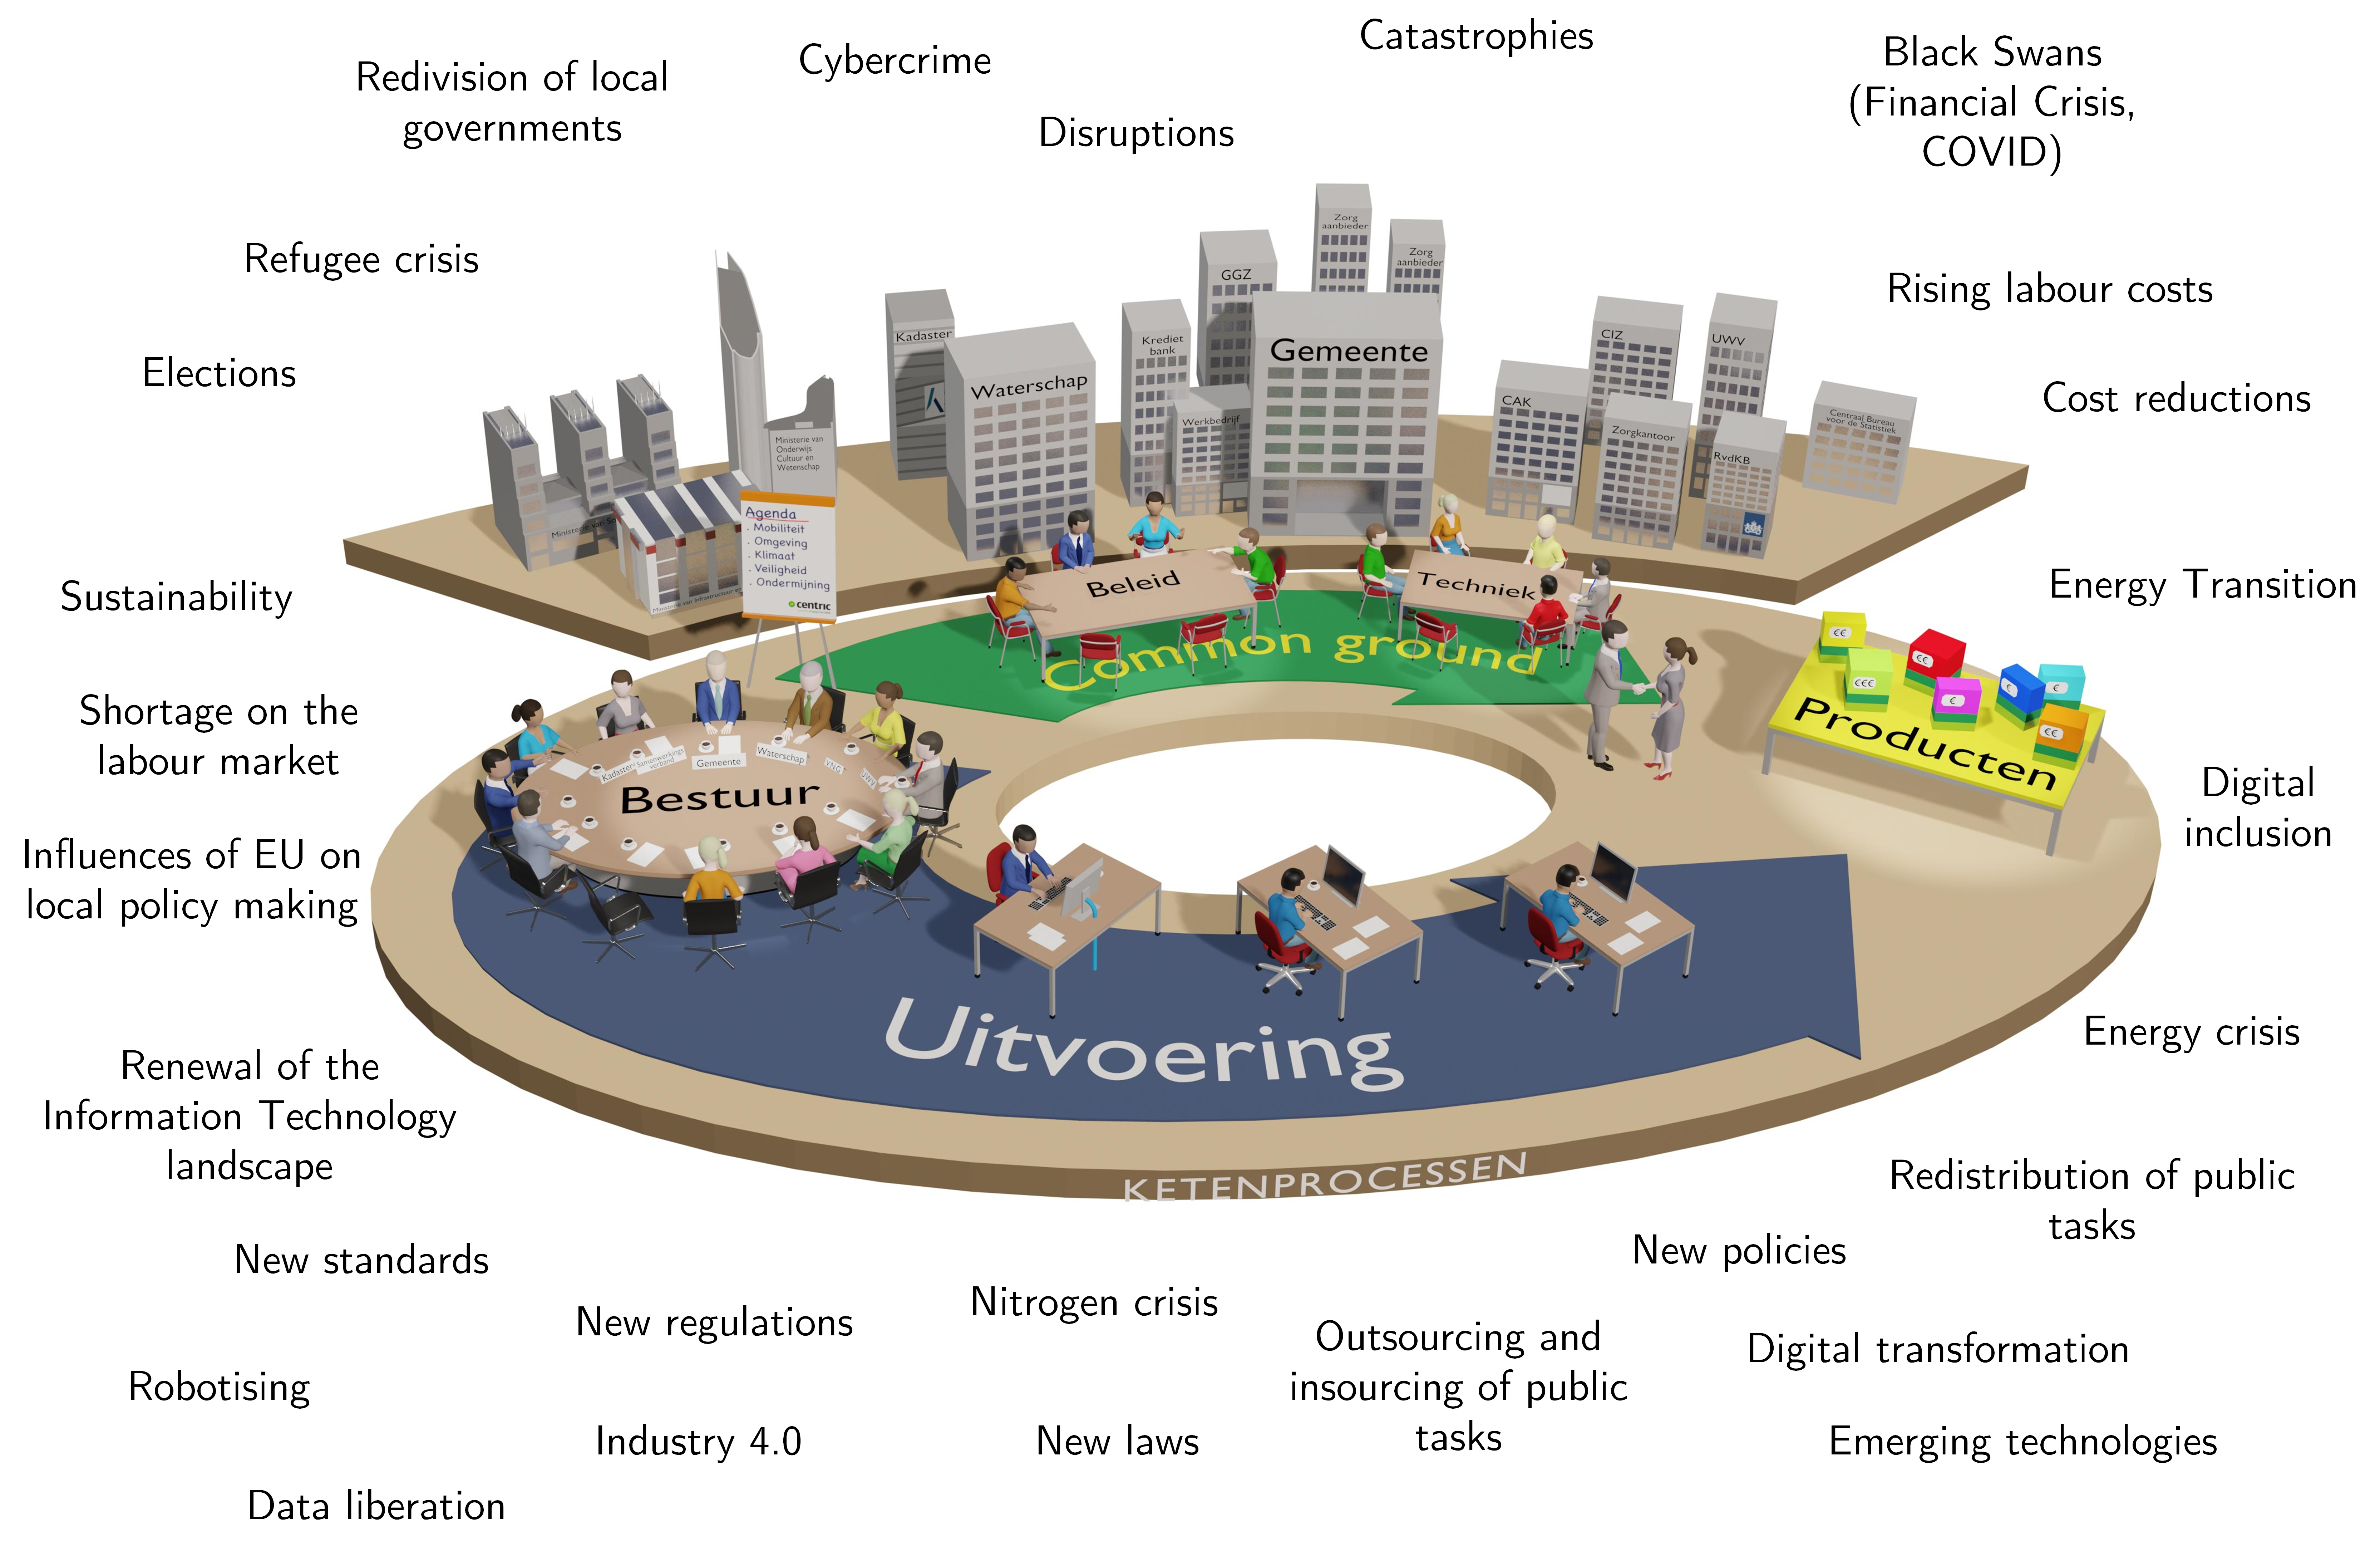
\includegraphics[width=0.8\linewidth]{images/publicstressors}
	\caption[Examples of stressors on the public sector]{Examples of stressors on the public sector}
	\label{fig:publicstressors}
\end{figure}
Because of the \gls{digitaltransformation}, the pace of change is increasing rapidly. In a study by \textcite{Eggers2015}, 96\% of respondents said digital technologies are significantly disrupting the \gls{ps}. According to \textcite{Nurmi2021}, organisations in the public and private sectors alike face the need to manage themselves in an ever more interconnected and fast-paced world. \textcite{Guggenberger2020} states that a paradigmatic change from a mechanistic toward a systemic worldview is ongoing, emphasizing the interconnectedness of participating organizations. 

\begin{remark}
	''The processes, while solid, cannot withstand the current pace of change; the dependence on emergency solutions and manual work is increasing'' \parencite[p.~2]{Wiebes2014}.
\end{remark}

The \gls{digitaltransformation} is not the only \gls{stressor} on the \gls{ps}. There are a lot of internal and external \glspl{stressor}. By being more \gls{robust} or \gls{resilient}, you can only withstand the change or the \gls{stressor}, but you do not gain from it. Governmental organisations and agencies in the Dutch \gls{ps} are searching for methods of dealing with this increased pace and the stressors. There are a lot of indications of this in the discussions and sessions held at \textcite{iBestuurterugblik2021}. The relevance of this research is not only about adding to the \acrshort{bok} of \acrshort{ea} and \gls{complexityscience} but also, in the context of public responsibility, to share the outcome with the \gls{ps} for further study and use.

\section{Design of the thesis}
\label{sec:structure}
The structure of this thesis follows a pattern of divergence before convergence (\cref{fig:design}). We introduce the research (\cref{ch:introduction}). We present the context, explain the design of the thesis, and the necessity of the research. Following, we introduce the main concepts of the research together with a problem statement and research questions. We give a background on the concepts of the research (\cref{ch:theoreticalbackground}). This part also contains the outcome of the literature research we performed based on the approach described in the methodology (\cref{ch:methodology}). The methodology explains the research design, the methods, the quality and the approach. All of these are part of the divergence of the research. We collected much data, but we still have to validate the data and narrow it down to formulate an answer to our research question. The second part of the thesis design will converge the findings.
\begin{figure}[H]
	\centering
	\includegraphics[width=0.9\linewidth]{images/structure}
	\caption[Design of the thesis]{Structure of the thesis}
	\label{fig:design}
\end{figure}
We validate findings with interviews (\cref{ch:interviews}) and an expert group (\cref{ch:expertgroup}). Converging ends with  conclusion and discussions (\cref{ch:conclusionanddiscussions}). The final part of the thesis design is a retrospective of the researcher, the research, and its process (\cref{ch:retrospective}). We have a glossary of terms available at the tail of the thesis to support the reader with used definitions.
 			%	Add the introduction
	\chapter{Theoretical background}
\label{ch:theoreticalbackground}

\section{What is a system?}
\label{sec:tbsystem}

\section{Organisation}
\label{sec:tborganisation}

\subsection{Independent Software Vendor}
\label{sub:tbisv}
\lipsum[1]

\section{antifragile}
\label{sec:tbantifragile}
\lipsum[1]

\begin{itemize}
	\item{Randomness}
	\item{Variability}
	\item{Hormesis / Mithridatisation (by taleb) / Antidotum Mithridatium}
\end{itemize}

\subsection{Relation of Antifragile with Robust, Resilient, and Agility}
\label{sub:tbrelatedtoantifragile}
\lipsum[1]

\section{VUCA}
\label{sec:tbvuca}
\lipsum[1]

\section{Enterprise Architecture}
\label{sec:tbea}
\lipsum[1]

\section{Public Sector market}
\label{sec:tbpsmarket}
\lipsum[1]

\section{What is a stressor?}
\label{sec:stressor}
\lipsum[1]


 				%	Add the Theoretical Background
	\chapter{Research Methodology}
\label{ch:research-methodology}

\section{Research Model}
\label{sec:research-model}
	\begin{figure}[h]
		\centering
		\includegraphics[width=12cm]{images/research-model.png}
		\caption[Research Model]{Research Model}
		\label{fig:research-model}
	\end{figure}

\section{Delphi Group}
For the Delphi Group participants see appendix~\ref{app:delphigroupparticipants} \\%

What about the sample size? Normally Delphi is about 100+. What about this research. How large should the sample size be for a qualitative result?

\section{Quality of the Research (old example text)}
\label{sec:quality-of-the-research}
The research was qualitative. The information is based on qualitative information gathered by the researcher
from employees of the organisation. However, with the research approach and transparency, the research can
be validated, can be repeated, so it is reliable and reducible. With the use of managerial models and methods
like Lean, Value Stream Mapping with supporting tools like NEN-ISO/IEC 25011 and ServQual got a nonbiased
result.\\
\begin{itemize}
	\item{\textbf{The validity} of the research is dependent on the right use of the right models and the right methods. The researcher conducted research on which models, frameworks and tools to use. The results and the rationales around the choice of theories, models, frameworks and tools are stated in chapter 4. The sources used for determining the theories, models, frameworks and tools are from scientific and expert sources.}
	\item{\textbf{The reliability} is about the influence of possible errors. For the research, the researcher used methods like triangulation, and sources from scientific reports and expert literature. The number of interviews was too small for the right statistical outcome. To enlarge the reliability of the interviews, the researcher used the same framework of themes for his semi-structured interviews. The transcriptions are placed in the appendixes for transparency. The information gathered with the interviewees is compared with the other interviewees.}
	\item{\textbf{The repeatability} is about getting the same results when the research is conducted again. The researcher uses his research design and research approach, as stated. All the steps taken are put into the research design. If this research design is followed, the same results should follow.}
	\item{\textbf{The reducibility} is about the outcome of the research can be deducted step by step. By using the research model, and the structure of the thesis, every step is reducible.}
\end{itemize}

\begin{itemize}
	\item{Think about Replication}
	\item{Recker types}
	\item{OpenScience}
	\item{Howto falsify?}
	\item{Rigourness}
\end{itemize}


\section{Used research tooling}

\LaTeX\ with the KOMA-Script Report template\\
TeXstudio\footnote{https://www.texstudio.org/}\\
TeX Live\footnote{https://tug.org/texlive/}\\
Dropbox\footnote{https://www.dropbox.com/}\\
GitHub\footnote{https://github.com/} (2 repositories) \\
	Master Thesis Repository\footnote{https://github.com/JRBliekendaal/master-thesis}\\
	Master Thesis Administration Repository\footnote{https://github.com/JRBliekendaal/master-thesis-administration}\\
GitHub Desktop\footnote{https://desktop.github.com/}\\
JabRef\footnote{https://www.jabref.org/} as a reference manager including integration with web browsers\\
PaperPanda\footnote{https://paperpanda.app/} for finding hard to find resources\\
Grammarly\footnote{https://www.grammarly.com/}

Microsoft Excel\\
Microsoft Powerpoint\\
Microsoft Visio\\
Sparx Enterprise Architect\\


Researchgate\\
Web of Science\\
Google Scholar\\
Meetingwizard\footnote{https://www.meetingwizard.nl/}\\


Hardware\\
Dell Windows PC with Windows 10\\
Amazon Kindle Oasis\\

leuchtturm1917 notebooks\\
				%	Add the methodology
	\chapter{Attributes}
\label{ch:attributes}

\section{Attributes of antifragile}
\label{sec:attributesantifragile}

\begin{figure}[h!]
	\centering
	\includegraphics[width=0.8\linewidth]{images/eaalbwincludingoptionality}
	\caption[Extended Antifragile Attribute List \parencite{Botjes2021} with Optionality]{Extended Antifragile Attribute List \parencite{Botjes2021} with Optionality}
	\label{fig:eaalbwincludingoptionality-attributes}
\end{figure}

\subsection{\Gls{attenuatevariety} attributes}
\begin{table}[H]
	\begin{center}
			\begin{tabular}{@{}ll@{}}
			\toprule
				\textbf{Attribute} & \textbf{Sources} \\%
				\midrule%
				Top Down C\&C & \parencite{Botjes2020} \\%
				Micro-Management & \parencite{Botjes2020} \\%
				Redundancy & \parencite{Botjes2020} \\%
				Modularity & \parencite{Botjes2020} \\%
				Loosely coupled & \parencite{Botjes2020} \\%
			\bottomrule%
			\end{tabular}
			\caption[Attenuating attributes of \gls{antifragile}]{Attenuating attributes of \gls{antifragile}}
			\label{tab:attenuatingattributes}
\end{center}
\end{table}				

\subsection{\Gls{amplifyvariety} attributes}
\begin{table}[H]
	\begin{center}
		\begin{tabular}{@{}ll@{}}
			\toprule
			\textbf{Attribute} & \textbf{Sources} \\%
			\midrule%
			\Gls{diversity} & \parencite{Botjes2020} \\%
			\Gls{optionality} & \parencites{Taleb2012}{Gorgeon2015} \\%
			\Gls{nonmonotonicity} & \parencite{Botjes2020} \\%
			\Gls{emergence} & \parencite{Botjes2020} \\%
			\Gls{selforganisation} & \parencite{Botjes2020} \\%
			\Gls{insertlowlevelstress} & \parencite{Botjes2020} \\%
			\Gls{networkconnections} & \parencite{Botjes2020} \\%
			\Gls{failfast} & \parencite{Botjes2020} \\%
			\Gls{resourcestoinvest} & \parencites{Taleb2012}{Botjes2020} \\%
			\Gls{senecabarbell} &  \parencites{Taleb2012}{Botjes2020} \\%
			\Gls{insertrandomness} & \parencites{Taleb2012}{Botjes2020} \\%		
			\Gls{reducenaiveintervention} & \parencites{Taleb2012}{Botjes2020} \\%
			\Gls{skininthegame} & \parencites{Taleb2012}{Botjes2020} \\%
			\bottomrule%
		\end{tabular}
		\caption[Amplifying attributes of \gls{antifragile}]{Amplifying attributes of \gls{antifragile}}
		\label{tab:amplifyingattributes}
	\end{center}
\end{table}			

\subsection{\Gls{attenuatevariety} and \gls{amplifyvariety} attributes}

\begin{table}[H]
	\begin{center}
		\begin{tabular}{@{}ll@{}}
			\toprule
			\textbf{Attribute} & \textbf{Sources} \\%
			\midrule%
			\Gls{personalmastery} & \parencite{Botjes2020} \\%
			\Gls{sharedmentalmodels} & \parencite{Botjes2020} \\%
			\Gls{buildingsharedvision} & \parencite{Botjes2020} \\%
			\Gls{teamlearning} & \parencite{Botjes2020} \\%
			\Gls{systemsthinking} & \parencite{Botjes2020} \\%
			\bottomrule%
		\end{tabular}
		\caption[Attenuating and amplifying attributes of \gls{antifragile}]{Attenuating and amplifying attributes of \gls{antifragile}}
		\label{tab:attenuatingandamplifyingattributes}
	\end{center}
\end{table}	

\section{Attributes of Enterprise Architecture}
\label{sec:attributesonea}

\subsection{Enterprise IT Architecting attributes}
\label{sub:enterpriseitarchitecting}
\begin{table}[H]%
	\begin{center}%
		\begin{tabular}{@{}ll@{}}%
			\toprule%
			\textbf{Attribute} & \textbf{Sources} \\%
			\midrule%
			 & \parencite{Lapalme2012} \\%
			\bottomrule%
		\end{tabular}%
		\caption[Attributes of Enterprise Ecological Adaptation]{Attributes of Enterprise Ecological Adaptation}%
		\label{tab:attributesofenterpriseitarchitecting}%
	\end{center}%
\end{table}%


\subsection{Enterprise Integrating attributes}
\label{sub:attributesofenterpriseintegrating}
\begin{table}[H]%
	\begin{center}%
		\begin{tabular}{@{}ll@{}}%
			\toprule%
			\textbf{Attribute} & \textbf{Sources} \\%
			\midrule%
			 & \parencite{Lapalme2012} \\%
			\bottomrule%
		\end{tabular}%
		\caption[Attributes of Enterprise Integrating]{Attributes of Enterprise Integrating}%
		\label{tab:attributesofenterpriseintegrating}%
	\end{center}%
\end{table}%

\subsection{Enterprise Ecological Adaptation attributes}
\label{sub:enterpriseecologicaladaptation}

\begin{table}[H]
	\begin{center}
		\begin{tabular}{@{}ll@{}}
				\toprule
				\textbf{Attribute} & \textbf{Sources} \\%
				\midrule%
				\Gls{systeminenvironment} & \parencite{Lapalme2012} \\%
				\Gls{holisticsystemicstance} & \parencite{Lapalme2012} \\%
				\Gls{intraorganisationalcoherency} & \parencite{Lapalme2012} \\%
				\Gls{organisationallearning} & \parencite{Lapalme2012} \\%
				\Gls{environmentallearning} & \parencite{Lapalme2012} \\%
				\Gls{systeminenvironmentcoevolutionlearning} & \parencite{Lapalme2012} \\%
				\bottomrule%
			\end{tabular}
		\caption[Attributes of Enterprise Ecological Adaptation]{Attributes of Enterprise Ecological Adaptation}
		\label{tab:attributesofeea}
	\end{center}
\end{table}


				%	Add chapter on EAAF Attributes
	\chapter{Interview results}
\label{ch:interviewresults}

\section{Interviews}
\label{sec:interviews}
The interviews are in the format of semi-structured. I used a minimal set of questions. Based on the answers, the technique of hitchhiking was applied when there was a suspicion of extra information about \acrshort{ea} and \gls{antifragile} attributes. The interview summaries can be found in \cref{app:interviewsummaries}.

\begin{table}[!h]
	\label{tab:interviewquestions}
	\begin{center}
			\begin{tabular}{@{}p{0.1\textwidth}p{0.75\textwidth}p{0.15\textwidth}@{}}
				\toprule
				\textbf{Number} & \textbf{Question} & \textbf{Concept} \\ \midrule %
				1a. & How is your organisation applying \acrshort{ea}? & \acrshort{ea} \\%
				1b. & Who is accountable for \acrshort{ea} in your organisation? & \acrshort{ea} \\%
				1c. & How is \acrshort{ea} enabling your organisation to quickly adapt to changes (external influences)? & \acrshort{ea} \\%
				2a. & Does the operational model of the\gls{ps} \gls{foster} \gls{agility}? & \Gls{antifragile} \\%
				2b. & How is the \acrshort{ea} of your organisation contributing to \gls{foster} \gls{agility} in the \gls{ps}? & \acrshort{ea} \\%
				3a. & How does the public sector deal with \gls{uncertainty}? & \Gls{antifragile} \\%
				3b. & How is the \acrshort{ea} of your organisation contributing to dealing with \gls{uncertainty} in the \gls{ps}?
				 & \acrshort{ea} \\%
				4a. & How is the public sector dealing with unexpected events? & \Gls{antifragile} \\%
				4b. & How is \acrshort{ea} of your organisation contributing to dealing with unexpected events in the \gls{ps}? & \acrshort{ea} \\%
				5a. & Could you describe the risk appetite of the \gls{ps}? & \Gls{antifragile} \\%
				5b. & How does the \acrshort{ea} of your organisation match the risk appetite of the \gls{ps}?
				  & \acrshort{ea} \\%
				6a. & How is \gls{diversity} and \gls{optionality} used in the \gls{ps}? & \Gls{antifragile} \\%
				6b. & How does \acrshort{ea} of your organisation support \gls{diversity} and \gls{optionality} in the \gls{ps}? & \acrshort{ea} \\%																								
				Closing & Did you miss an important subject or do you want to add something else? & non-specific \\%
				\bottomrule
			\end{tabular}
		\caption{Interview questions}
	\end{center}
\end{table}

\section{Summary of interviews}


\section{Identified success factors}

\label{sec:interviewidentifiedsuccessfactors}
\begin{table}[!h]
	\begin{center}
		%\resizebox{\textwidth}{!}{%
			\begin{tabular}{@{}llllll@{}}
				%\toprule
				\textbf{Attribute} & \textbf{Behaviour} & \rot{90}{\textbf{Central Government}} & \rot{90}{\textbf{Local Government}} & \rot{90}{\textbf{Independent Software Vendor}} & \rot{90}{\textbf{Service Provider}} \\ \midrule
				Top Down C\&C & Engineering Resilience & \checkmark & \checkmark & \checkmark & \checkmark \\
				Micro-Management & Engineering Resilience & & & & \\
				Redundancy & Systems Resilience & & & & \\
				Modularity & Systems Resilience & & & & \\
				Loosely coupled & Systems Resilience & & & & \\
				Diversity & \acrshort{cas} Resilience & & & & \\
				Optionality & \acrshort{cas} Resilience & & & & \\
				Non-Monotonicity & \acrshort{cas} Resilience & & & & \\
				Emergence & \acrshort{cas} Resilience & & & & \\
				Self-Organisation & \acrshort{cas} Resilience & & & & \\
				Insert low-level stress & \acrshort{cas} Resilience & & & & \\
				Network-connections & \acrshort{cas} Resilience & & & & \\
				Fail Fast & \acrshort{cas} Resilience & & & & \\
				\Gls{resourcestoinvest} & Antifragile & & & & \\
				\Gls{senecabarbell} & Antifragile & & & & \\
				\Gls{insertrandomness} & Antifragile & & & & \\			
				\Gls{reducenaiveintervention} & Antifragile & & & & \\
				\Gls{skininthegame} & Antifragile & & & & \\
				\Gls{personalmastery} & Learning Organisation & & & & \\
				\Gls{sharedmentalmodels} & Learning Organisation & & & & \\
				\Gls{buildingsharedvision} & Learning Organisation & & & & \\
				\Gls{teamlearning} & Learning Organisation & & & & \\
				\Gls{systemsthinking} & Learning Organisation & & & & \\
				\bottomrule
			\end{tabular}
		%}
		\caption{Identified success factors from interviews}
	\end{center}
\end{table}				%	Interview results
	\chapter{Expert group}
\label{ch:expertgroup}
\setcounter{footnote}{0}
In \cref{ch:interviews}, the \glspl{attribute} were selected. The selected \glspl{attribute} are most likely to have a positive influence on \acrshort{ea} in achieving \gls{antifragility} in the \gls{ps}. These attributes are the result of literature study (\cref{ch:attributes}) and the qualitative analysis of interviews (\cref{ch:interviews}). The \glspl{attribute} still needed to be validated for \gls{triangulation} to work. An expert group validated these \glspl{attribute}. All of the expert group participants have experience with \acrshort{ea} and the \gls{ps}. A survey on experience was part of the expert group session (\cref{tab:experiencevalidationgroup}). The expert group participants were selected to balance the group. There was a balanced mix of participants from the central government, the local government, independent software vendors, service providers, and universities. Ten experts participated in the session.

The expert group session had a duration of 2 hours. The expert group session was online with Microsoft Teams and Meeting Wizard (a group support system). There is a recording and a transcription available of this session. All participants gave their consent. The transcription and recording are not publicly available because they cannot be anonymised\footnote{The Antwerp Management School can request the recordings and transcriptions only for (re)accreditations and visitations to enable the Antwerp Management School to comply with statutory obligations. The recordings and transcriptions are kept for seven years after graduation before being deleted.}.
\begin{table}[H]
	\centering
	\begin{tabular}{p{.55\textwidth}ccc}
		\toprule
		\textbf{Question} & \textbf{Years} & \textbf{Variability} & \textbf{Abstains} \\
		\midrule
		How many years of experience do you have in the field of enterprise architecture? & 9,8 & 8\% & 0 \\%
		How many years have you worked as an (enterprise) architect? & 10,6 & 12\% & 0 \\%
		How many years of experience do you have in the field of complexity sciences (like antifragile)? & 7,4 & 16\% & 0 \\%
		How many years of experience do you have with the public sector? & 12,2 & 17\% & 0 \\%
		How many years of experience do you have with working in publicly-held organisations? & 10 & 16\% & 0 \\%
		How many years of experience do you have with working in privately-held organisations? & 17,2 & 21\% & 0 \\%
		\bottomrule
	\end{tabular}%
	\caption[The average experience of expert group participants]{The average experience of expert group participants}
	\label{tab:experiencevalidationgroup}%
\end{table}%
All the participants received information beforehand by email. This information contained the invite, the goal of the session, the agenda and all relevant definitions. Three youtube videos\footnote{\url{https://www.youtube.com/watch?v=B2-QCv-hChY}, \url{https://www.youtube.com/watch?v=1NXaafTpVjM}, and \url{https://www.youtube.com/watch?v=C40zwpdc_yo}} were shared to ensure that the participants had a basic understanding of \gls{antifragility}. All participants confirmed that they did see at least one of the videos. There were also multiple participants who read the book of \textcite{Taleb2012}. For the session the following agenda was used:
\begin{enumerate}
	\item{Introduction}
	\item{Survey on experience\footnote{for the outcome of this survey see \cref{tab:experiencevalidationgroup}}}
	\item{Presentation on the results of the research up to now\footnote{\url{https://github.com/JRBliekendaal/master-thesis/blob/main/datasets/expertgroup/validationsession.pdf}}}
	\item{Validation of attributes and ea school of thought}
	\item{Survey on the relevance of the research}
\end{enumerate}
Meeting Wizard supported the survey's and the validations. The output from these 




\section{Expert group validation}
\label{sec:expertgroupvalidation}

the two newly found attributes \gls{adapttobusinesslanguage} and \gls{safeworkingenvironment} were logically placed with the categories antifragile and Enterprise Architecture attributes. \Gls{adapttobusinesslanguage} had something to do with enterprise architecture and safe working environment had more to do with the antifragile attributes.


\subsection{Validation of antifragile attributes}
\label{sub:validationofantifragileattributes}

\begin{table}[H]
	\centering
	\begin{tabular}{p{.55\textwidth}ccc}
		\toprule
		\textbf{Attribute} & \textbf{Rating} & \textbf{Variability} & \textbf{Abstains} \\
		\midrule
		Optionality & 6,9 & 32\% & 0 \\%
		Mono-Monotonicity & 7 & 51\% & 0 \\%
		Self-Organisation & 8,2 & 23\% & 0 \\%
		Fail-Fast & 7,8 & 35\% & 0 \\%
		Resources to Invest & 6,7 & 36\% & 1 \\%
		Seneca's Barbell & 5,8 & 37\% & 1 \\%
		Safe working environment & 7,4 & 31\% & 0 \\%
		Naar buiten kijken, samenwerking zoeken & 6,2 & 55\% & 0 \\%
		Data Governance planes (tbv infrastructure-as-code / Software Defined Anything) & 4,4 & 56\% & 1 \\%
		\bottomrule
	\end{tabular}%
	\caption{Validation of antifragile attributes}
	\label{tab:validationofantifragileattributes}%
\end{table}%


\subsection{Validation of Enterprise Architecture attributes}
\label{sub:validationofenterprisearchitectureattributes}




\section{title}

				%	Add expert group chapter
	\include{contents/analysis}					%	Add Analysis Chapter
	\chapter{Conclusion and discussions}
\label{ch:conclusionanddiscussions}

\lipsum[1]




\section{Conclusion}
\label{sec:conclusion}

\lipsum[1]

\section{Discussions}
\label{sec:discussions}

\begin{itemize}
	\item{Discuss the definition of System Thinking vs Emergence}
	\item{Discuss Blaming Culture Public Sector}
	\item{Discuss Speaking the language of the Business with EA}
\end{itemize}

\section{Recommendations}
\label{sec:reccomandations}

\lipsum[1]
				%	Add the conclusion
	\chapter{Retrospective}
\lipsum[1]

\begin{itemize}
	\item{The added value of a Co-Promotor}
\end{itemize}
			%	Add the restrospective
	
	% Tail of Thesis

	\printbibliography[title={References}]			%	Add Bibliography
	\newpage										%
	\listoffigures									%	Add the List of Figures
	\addcontentsline{toc}{chapter}{List of Figures} % Add List of Figures to Table of Contents
	\newpage										%			
	\listoftables									%	Add the list of Tables
	\addcontentsline{toc}{chapter}{List of Tables} 	% Add List of Tables to Table of Contents
	\printglossary[title=Glossary of Terms] 		% Add Glossary of Terms
	\printglossary[type=\acronymtype,title=Abbreviations] % Add Abbreviations

	\begin{appendices}	% Add Appendices
	%	\chapter{Personal Motivation}
I always want to know how something works and why it works the way it works. This eagerness started at a very early age. I always demolished birthday presents into their parts. I wondered how things worked, and I did not stop with the research on the how and why until I understood it. The search for the how and why is a central theme in my life. And because of this, I never stopped learning. When the why is not known, I never give up researching—not knowing the why has only the meaning that nobody has found the answer yet. 

My essential attitude is that of a mathematician or a scientist. I am very binary and sceptical when something is somewhere in between, and I am not fond of shades of grey. So clear definitions is what I pursue. Everything needs an explanation. When I cannot explain, I do not fall back to religion, infinity, approximately, or even ''it is just what it is''. I only accept that we did not find the answer yet.

This journey started with simple things like a toy car or a doll that had a mechanism of saying things. I still think of my little sister, who found hers back in tiny pieces. Later the subjects of research began to be different. Secondary education drove me to understand chemistry, physics, and biology, and I needed an explanation on the who and why to understand it. This drive was probably the main reason I was not perfect in languages. You cannot put consistent rules on languages.  Languages do not have a clear rationale for the rules, and I often heard it is just the way it is.

Grammar school taught me that I was a natural in research, and I decided to pursue research. Firstly at several Universities, but I failed big time. The Universities at that time gave me a lot of answers that it is the way it is, and most of the lecturers did not appreciate me challenging them on the why. Because of this, I started pursuing a job that could fulfil my eagerness for researching, and I found that with an IT Company in the Netherlands.

The technical (hard) side of IT was, at that time, a match made in heaven. Most of the time, it is just like math, you have a clear answer, and you know why you get that answer. Before I knew it, I was a Senior Consultant and an IT Architect shortly after that. Gaining knowledge is one thing that drives me, but the other thing is sharing that knowledge with others. Gaining and sharing knowledge is the thing that gets me up in the morning. For sharing knowledge, I taught, as a trainer, adults on the why and how of technology subjects for years.

In those years, I advised dozens of companies of the public and private sectors in the Benelux on how they could apply technologies and what problem it solved for them. This period did teach me a lot by seeing other companies and working with different kinds of people. But technology was driving me less and less. Most of the time technology did not change with new releases or new versions. In the base it was still the same mean to reach a business goal. I often solved my customers' problems by not introducing new technology but changing their processes, information architecture, culture, team compositions, or organisational construction. I became more and more interested in how and why organisations could achieve their goals by using IT.

I am very succesfull in this field of work but I always wondered why I did things in a certain way. This led my back to education and I started a Bachelor in Business \& IT with a University of Applied Sciences. This time it was a big success. Because I already had a lot of experience I was admitted to a University of Applied Sciences only for people who had already experience. They did expect me to challenge the teachers on the why.



		\chapter{Properties of the Enterprise Architecture schools of thought}
\label{app:easchoolsproperties}
\section{The properties of Enterprise IT Architecting}
\begin{small}
\begin{longtable}{p{.2\textwidth}p{.8\textwidth}}
	\toprule
	& \textbf{Enterprise IT Architecting school of thought} \\ \midrule%
	\endhead%
	\hline
	\caption{Properties of Enteprise IT Architecting \parencite[p. 39]{Lapalme2012}}
	\label{tab:enterpriseitarchitecting}	
	\endfoot%
	Motto    		& Enterprise architecture is the glue between business \& IT \\
	Objectives and 	& Effectivily enable the enterprise strategy \\
	concerns		& Support IT planning and reduce cost \\
					& Enable business \\
	Principles and  & Apply reductionist (mechanistic) stance \\
	assumptions		& Don't question business strategies  \\
					& Design organisational dimensions independently \\
					& Don't worry about non-IT dimensions; they are not your concerns \\
	Skills 			& Have technical competence and engineering knowledge \\
	Challenges		& Convince the organisation to accept the designed plans \\
	Insights		& Permits the design of robust and complex technological solutions \\
					& Fosters the creation of high-quality models and planning scenarios \\
	Limitation		& Can produce inadequate or unfeasible solutions for the larger organizational context \\
					& Struggles with solution acceptance and implementation barriers \\
					& Susceptible to “perfect” designs 	that support unsustainable strategies \\
	\bottomrule
\end{longtable}
\end{small}
\newpage
\section{The properties of Enterprise Integrating}
\begin{small}
\begin{longtable}{p{.2\textwidth}p{.8\textwidth}}
	\toprule
	& \textbf{Enterprise Integrating school of thought} \\ \midrule%
	\endhead%
	\hline
	\caption{Properties of enterprise integrating \parencite[p. 39]{Lapalme2012}}
	\label{tab:interpriseintegrating}	
	\endfoot%
	Motto    		& Enterprise architecture is the link between strategy and execution \\
	Objectives and 	& Effectively implement the enterprise strategy \\
	concerns		& Support organizational coherence \\
	Principles and  & Apply a holist (systemic) stance \\
	assumptions		& Don’t question business strategies and objectives  \\
					& Manage the environment \\
					& Jointly design all organisational dimensions \\
	Skills 			& Facilitate small-group collaboration \\
					& Apply systems thinking \\
	Challenges		& Understand organizational systemic dynamics \\
					& Collaborate across the organization \\
					& Encourage systems thinking and paradigm shifts \\
	Insights		& Permits the design of comprehensive solutions \\
					& Enables significant organizational efficiency by eliminating unnecessary contradictions and paradoxes \\
	Limitation		& Susceptible to “perfect” designs that support unsustainable strategies \\
					& Requires a paradigm shift from reductionism to holism \\
	\bottomrule
\end{longtable}
\end{small}
\newpage
\section{The properties of Enterprise Ecological Adaptation}
\label{appsec:eea}

The properties of an \acrshort{eea} are:

\begin{small}
\begin{longtable}{p{.2\textwidth}p{.8\textwidth}}
	\toprule
	& \textbf{\acrlong{eea} school of thought} \\ \midrule%
	\endhead%
	\hline
	\caption{Properties of \acrlong{eea} \parencite[p. 39]{Lapalme2012}}
	\label{tab:eaeea}	
	\endfoot%
	Motto    		& Enterprise architecture is the means for organizational innovation and sustainability \\
	Objectives and 	& Innovate and adapt    \\
	concerns		& Support organizational coherence \\
					& Encourage system-in-environment coevolution \\
	Principles and  & Apply a holist (systemic) stance \\
	assumptions		& System-in-environment coevolution  \\
					& Environment can be changed \\
					& Jointly design all organisational dimensions \\
	Skills 			& Foster dialogue \\
					& Apply system and system-in-environment thinking \\
					& Facilitate larger-group collaboration \\
	Challenges		& Foster sensemaking \\
					& Encourage systems thinking and systems-in-environment paradigm shifts \\
					& Collaborate across the organisation \\
	Insights		& Fosters system-in-environment coevolution and enterprise choherency \\
					& Fosters organisational innovation and sustainability \\
	Limitation		& Requires many organisational preconditions for management and strategy creation \\
	\bottomrule
\end{longtable}
\end{small} % Add EA Schools of thought of Lapalme details
		\chapter{Authors of the Enterprise Architecture schools of thought}
\label{app:easchoolsresearchers}

\textcite[p. 42]{Lapalme2012} Mapping enterprise architecture authors according to the three schools of thought.
\begin{small}
\begin{longtable}{p{.33\textwidth}p{.33\textwidth}p{.33\textwidth}}
	\toprule
	\textbf{Enterprise IT Architecting}	& \textbf{Enterprise Integrating} & \textbf{Enterprise Ecological Adaption} \\ \midrule%
	\endhead%
	\hline
	\caption{Authors of the Enterprise Architecture schools of thought \parencite[p. 42]{Lapalme2012}}
	\label{tab:easchoolresearchers}	
	\endfoot%
	Clive Finkelstein				&		Peter Bernus and Colleagues (editors)	&		Jamshid Gharajedaghi \\
	Inge Hanschke					&		Ronald Giachetti						&		Tom Graves \\
	Col Perks and Tony Beveridge	&		Leon Kappelman (editor)					&		Jan Hoogervorst \\
	Jeanne Ross and colleagues		&		Martin Op't Land and colleagues			&		James Martin \\
	Steven Spewak and Steven Hill	&												&		Kevin Smith and Tom Graves \\
	Martin van den Berg and Marlies van Steenbergen & 								&		James Lapalme and Donald de Guerre \\
	\bottomrule
\end{longtable}
\end{small} % Add writers per school of thought of Lapalme
	%	\chapter{Overview of Laws}
\setcounter{footnote}{0}
The research references to several laws. This appendice gives a small explainatory overview of these laws.

\begin{itemize}
	\item{2\textsuperscript{nd} Law of Thermodynamics}
	\item{Conways Law}
	\item{Metcalfe's Law}
	\item{Law of Municipalities}
\end{itemize}

\section{2\textsuperscript{nd} Law of Thermodynamics}
\label{sec:appendix2ndlawthermodynamics}
The ‘2\textsuperscript{nd} Law’ was formulated after nineteenth century engineers noticed that heat cannot pass from a colder body to a warmer body by itself. It states that in any closed system the amount of order can never increase, only decrease over time. Another way of saying this is that entropy always increases.

\section{Conway's Law}
Any organization that designs a system (defined broadly) will produce a design whose structure is a copy of the organization's communication structure.

\section{Metcalfe's Law}
Metcalfe's Law\footnote{\url{https://www.techopedia.com/definition/29066/metcalfes-law}} states that a network's impact is the square of the number of nodes in the network. For example, if a network has 10 nodes, its inherent value is 100 (10 * 10). The end nodes can be computers, servers and/or connecting users.

\section{Thorbecke's Law}

\section{Lehman's Law of Increasing Complexity}
As an evolving program is continually changed, its complexity, reflecting deteriorating structure, increases unless work is done to maintain or reduce it.


		\chapter{Conceptmap of antifragile attributes}
\label{app:cmapafattributes}

\begin{sidewaysfigure}
	\centering
	\includegraphics[width=0.9\linewidth]{images/cmapafattributes}
	\caption{Concept map of Antifragile Attributes}
	\label{fig:conceptmapafattributes}
\end{sidewaysfigure}
		\appendix
\chapter{Literature catch-up}
\label{app:literaturecatchup}
This appendix contains the newly found literature as a catch-up on the literature research of \textcite{Botjes2020}.

\begin{longtable}{p{.4\textwidth}p{.4\textwidth}p{0.1\textwidth}}
	\toprule%
	\textbf{Title} & \textbf{Author} & \textbf{Year} \\
	\midrule%
	\endhead%
	\hline
	\endfoot%
	\caption[Literature search 2020--March 2022 all sources]{Literature search 2020--March 2022 all sources}
	\label{tab:literatureafter2020all}
	\endlastfoot%
		A Barbell Strategy-oriented Regulatory Framework and Compliance Management & Gallina, Barbara & 2020 \\
		A collaborative approach to resilient and antifragile business ecosystems & Ramezani, Javaneh and Camarinha-Matos, Luis M. & 2019 \\
		A Game Theoretic Approach for Quality Assurance in Software Systems Using Antifragility-Based Learning Hooks & Vimaladevi, M. and Zayaraz, G. & 2020 \\
		A Literature Review of Organizational Resilience & Ping, Li Peter and Jiazhe, Zhu & 2021 \\
		A Philosophy of Security Architecture Design & Koien, Geir M. & 2020 \\
		Agile architecture & Kruchten, Philippe & 2013 \\
		An Introduction to Residuality Theory: Software Design Heuristics for Complex Systems. & O'Reilly, Barry M. & 2020 \\
		Antifragility as a design criterion for modelling dynamic systems & de Bruijn, Harald and Groessler, Andreas and Videira, Nuno & 2020 \\
		Approaches for resilience and antifragility in collaborative business ecosystems & Ramezani, Javaneh and Camarinha-Matos, Luis M. & 2020 \\
		Architecture Principles for Resilience & Furrer, Frank J & 2019 \\
		Beyond Resilience in Sociotechnical Systems & Simonette, Marcel and Magalhaes, Mario and Bertassi, Eduardo and Spina, Edison & 2019 \\
		Black-Swan Type Catastrophes and Antifragility/Supra-resilience of Urban Socio-Technical Infrastructures & Timashev, S. A. & 2020 \\
		Conceptualizing resilience in engineering systems: An analysis of the literature & Wied, Morten and Oehmen, Josef and Welo, Torgeir & 2020 \\
		Cybersecurity in the Internet of Things in Industrial Management & Raimundo, Ricardo Jorge and Rosario, Alberico Travassos & 2022 \\
		Ecosystem antifragility: beyond integrity and resilience & Equihua, Miguel and Espinosa Aldama, Mariana and Gershenson, Carlos and Lopez-Corona, Oliver and Munguia, Mariana and Perez-Maqueo, Octavio and Ramirez-Carrillo, Elvia & 2020 \\
		Emerging risk management in industry 4.0: an approach to improve organizational and human performance in the complex systems & Brocal, Francisco and Gonzalez, Cristina and Komljenovic, Dragan and Katina, Polinpapilinho F and Sebastian, Miguel A & 2019 \\
		Enterprise Architecture Resilience by Design: A Method and Case Study Demonstration & Aldea, Adina and Vaicekauskaite, Egle and Daneva, Maya and Piest, Jean Paul Sebastian & 2021 \\
		Enterprise Development Management through managed chaos & Kasianova, Nataliia and Tarasova, Elena and Kravchuk, Nataliia & 2019 \\
		Facing uncertainty: An entrepreneurial view of the future? & Bridge, Simon & 2021 \\
		Microservice Architecture & Nadareishvili, Irakli and Mitra, Ronnie and McLarty, Matt and Amundsen, Mike & 2019 \\
		No More Snake Oil: Architecting Agility through Antifragility & O'Reilly, Barry & 2019 \\
		On the meaning and operationalization of antifragility: Comment on the paper by Grossler & van Daalen, Els & 2020 \\
		Resilience, robustness, and antifragility: Towards an appreciation of distinct organizational responses to adversity & Munoz, Albert and Billsberry, Jon and Ambrosini, Veronique & 2022 \\
		Self-Improving Autonomic Systems for Antifragile Cyber Defence: Challenges and Opportunities & Chhetri, Mohan Baruwal and Uzunov, V, Anton and Vo, Quoc Bao and Nepal, Surya and Kowalczyk, Ryszard & 2019 \\
		The Business Transformation Framework and Enterprise Architecture Framework for Managers in Business Innovation The role of legacy processes in automated business environments & Trad, Antoine and IBISTM, France and Kalpic, Damir & 2017 \\
		The Machine in the Ghost: Autonomy, Hyperconnectivity, and Residual Causality & O'Reilly, Barry M. & 2021 \\
		The Philosophy of Residuality Theory & O'Reilly, Barry M. & 2021 \\
		The Tao way to anti-fragile software architectures: the case of mobile applications & Grassi, Vincenzo and Mirandola, Raffaela & 2021 \\
		Toward a commonly shared public policy perspective for analyzing risk coping strategies & Li, Yanwei and Taeihagh, Araz and de Jong, Martin and Klinke, Andreas & 2021 \\
		Tutorial on systems with antifragility to downtime & Hole, Kjell Jorgen & 2022 \\
		We need more Anti-Fragility! & Dirzus, Dagmar & 2020 \\
	\bottomrule%
\end{longtable}

	%	\chapter{Interview Participants}
\label{app:interviewparticipants}

\begin{table}[!h]
	\begin{center}
		\begin{tabular}{@{}ccccc@{}}
			\toprule
			\textbf{Who} & \textbf{Role} & \textbf{From} \\ \midrule
			Christiaan Konstapel & Lead Enterprise Architect & Mileway \\
			Y    & 2    & tbd \\
			Y    & 2    & tbd \\ \bottomrule
		\end{tabular}
		\caption{Interview Participants}
		\label{tab:interviewparticipants}
	\end{center}
\end{table}
	%	\chapter{Delphi Group Participants}
\label{app:delphigroupparticipants}

\begin{table}[!h]
	\begin{center}
		\begin{tabular}{@{}ccccc@{}}
			\toprule
			\textbf{Who} & \textbf{Role} & \textbf{From} \\ \midrule
			Jan Ploeg & Enterprise Architect & Centric Netherlands B.V. (ISV) \\
			Y    & 2    & Other ISV \\
			Y    & 2    & Municipality \\
			Y    & 2    & VNG-Realisatie \\
			Y    & 2    & Logius \\
			Z    & 0    & Academic \\ \bottomrule
		\end{tabular}
		\caption{Delphi Group Participants}
		\label{tab:delphigroupparticipants}
	\end{center}
\end{table}
	%	\chapter{Literature Selection}
\label{app:literature_selection}


		\chapter{Interview summaries}
\label{app:interviewsummaries}
\section{Interview central government}
\label{sec:interviewcentralgovernment}
\subsubsection{Question 1 / Enterprise Architecture}
\acrshort{ea} is not used and we are not \gls{agile}. \acrshort{ea} is too difficult for the public administrators. In addition, we are also responsible for other sectors. There is not one architecture. We have multiple reference architectures. What we have to do in the public sector depends on the political decision making within the period of governing (four years until new elections). \acrshort{ea} is at the end of the chain of administrative decision-making.
\subsubsection{Question 2 / Agility of the public sector}
It is hard to be \gls{agile} within the \gls{ps}. Everything needs to be predefined and planned. \Gls{agile} working is very difficult within the government. The end goal is not very clear with \gls{agile} working. It is unclear how the public money is spent on precisely what. 
\subsubsection{Question 3 / Dealing with uncertainty and unexpected events}
The \gls{ps} cannot deal with \gls{uncertainty}. Everything must be predefined and planned. There must be accountability for how public money is spent. All missteps are magnified. There is a quick result in crises, but with possible consequences later on because of \acrfull{bit} audits or \glspl{parliamentaryinquiry}.
\subsubsection{Question 5 / The risk appetite of the public sector}
There is no risk appetite. Everything must be known and explainable in advance. If it is found that the procedures are not used, it can result in political consequences later on. Afterwards, positive lessons learned are not used to make adjustments within the public sector. Experimentation is (almost) not possible.
(note: blaming culture)
\subsubsection{Question 6 / Using diversity and optionality in the public sector}
It would be nice to work with optionality and smaller units within the \gls{ps} and \acrshort{ea} to make it easier to adapt. Think about in \acrshort{ea} disposable microservices. Nevertheless, it remains that \acrshort{ea} is not important. It is at the end of the chain and is not used in administrative decision-making. Enterprise architecture is confronted with decision-making.
\subsubsection{Closing statements}
\Gls{antifragile} is not directly applicable for the central government, but it can have a lot of benefits for suppliers in the \gls{ps}. Do not advertise it but exploit it to become better. In the case of an \acrfull{isv} think about many disposable microservices so it will be easier to deal with the \gls{ps}.
\section{Interview local government}
\label{sec:interviewlocalgovernment}
\subsubsection{Question 1 / Enterprise Architecture}
There is somewhat of an \acrshort{ea}, but we are not using it that broadly. As an organisation, we do not have a real \acrshort{ea}. Our organisation is best compared to that of a consultancy firm. Our core task is lobbying advocacy. We guide the things we do, and then again, it concerns the things we do for municipalities or on behalf of municipalities. We have a multi-year vision. We use guiding principles for the things we do.
Nevertheless, there are processes in the making for portfolio management. What do we do, what don't we do, and how do they relate to each other. There is not one responsibility on the \acrshort{ea}. It is a stepped responsibility that lies with committees and the services board. When it comes to IT, the responsibility lies with the Directory of Information Society. \acrshort{ea} is used for assay the request for subsidy. When there is a request for a subsidy that is not in line with the goals, it is not requested by the (European) government.
The case of how \acrshort{ea} contributes to the agility of the public sector is complicated. The public administrators are not architects and vice versa. \acrshort{ea} is hard to understand. \acrshort{ea} does not provide answers for the problems of today. Ultimately \acrshort{ea} should deliver this so the change can start tomorrow. It is essential to clarify the problems that public administrators are having. Both the facts as well the underlying causes. \acrshort{ea} should clarify the differences. Make it clear where we need to go and map out a path to get there, based on little steps that ultimately lead to the goal. Moreover, in the language public administrators understand. The architect must use the language of the stakeholders to make \acrshort{ea} successful (note: success factor).
\subsubsection{Question 2 / Agility of the public sector}
The \gls{ps} is more about risk aversion. Legality is about holding on to what is known. So, it is exactly known what the municipalities do, and we know precisely what the Land Registry does. All the subsystems of the \gls{ps} have a defined assignment. Moreover, it would be best if it stayed between the lines. Think, for example, about purpose limitation. Purpose Limitation will hold it back when \gls{ps} wants to be agile. The \gls{ps} cannot experiment that easily with rules like these. It will put experimentation at the edge.
The operating model of the \gls{ps} does not offer the freedom to do so that easily. The \gls{ps} can not experiment, discover and then say this was a nice experiment; let us go further. It is impossible to take decisions on the whole, such as within the social domain. If you have the right to confiscate a car, you cannot decide that there need to be a taxi to drive kids to school. It is a responsibility of a different part of the \gls{ps}. This all has to do with \gls{houseofthorbecke}\footnote{\url{https://www.denederlandsegrondwet.nl/id/vieqcpdzf0gw/bestuurlijke_indeling}} together with the current legislation and regulations. It does not mean that the \gls{ps} does not want to be more agile. It is not about separate parts of the government anymore. There is more and more collaboration based on federation. The \gls{ps} wants to be more agile. It is often a subject of conversation. Nevertheless, it gets stuck in the administrative decision-making processes.
\subsubsection{Question 3 / Dealing with uncertainty}
The reflex on \gls{uncertainty} of the \gls{ps} is that the \gls{ps} gets very insecure from \gls{uncertainty}. So the \gls{ps} does not know how to deal with \gls{uncertainty}. The common reflex is to push the uncertainty back to robust/resilient, so it is under control again. Robust \& resilient is back to its previous state but then sturdier, more robust (note: Risk avoidance). However, the \gls{ps} claims that they can deal with it. See, for example, the energy transition. The \gls{ps} defined the framework for this transition. It can contribute to the economy with many new jobs and a new knowledge model. We did see that also in the past with road and waterway engineering. Nevertheless, then they forget about the mechanisms needed to accomplish it. So the \gls{ps} does want to deal with \gls{uncertainty}, but the \gls{ps} is not creating the right conditions or the freedom of acting to be able to do so.
The available \acrshort{ea}'s within the \gls{ps} do not help either. It does not contribute to accept \gls{uncertainty}. At the most, our new vision on Information, Common Ground\footnote{\url{https://commonground.nl/}}, is contributing to this. An important principle in that vision is the ''community'' principle that could help with this \gls{uncertainty} (note: shared mental models). This principle states that municipalities, chain partners, market parties and the \acrshort{vngr} work together as a community in realisation. It is the certainty that it is uncertain. There are always new issues, and organising collaboration will help us to better deal with this \gls{uncertainty}, especially in the \gls{ps}.
\subsubsection{Question 4 / Dealing with unexpected events}
We, fortunately, live in a country where the \gls{ps} is staffed with good people who understand what citizens need or what is needed in a disaster area. So help is available pretty quickly. For example the fires at Moerdijk\footnote{\url{https://nl.wikipedia.org/wiki/Brand_Moerdijk_5_januari_2011}}, near Rotterdam. Or the plane crash of Turkish Airlines\footnote{\url{https://en.wikipedia.org/wiki/Turkish_Airlines_Flight_1951}} at Schiphol. Before we knew it, the fires were already distinguished. However, the \gls{ps} is not able to ascertain if it is an incident or a structural problem. If the problem takes too long, we see the reflex to control it again, so we fall back to our past habits. Adopting newly learned patterns is hard with the current legislation and regulations. Maybe we must be in a continuous crisis, so we have the freedom to do what we have to do. It is easier to be more agile in a crisis. With the local governments, there is only one who can decide what to do in a crisis, and this is the mayor as part of the triangle\footnote{\url{https://nl.wikipedia.org/wiki/Driehoek_(overheid)}}. 
It seems that the local governments have two organisation \& operational models. A model for running the municipality in a normal state and one in a state of crisis. (note: Seneca's Barbell?)
\subsubsection{Question 5 / The risk appetite of the public sector}
Drive and urge for innovation and change, which could perhaps be another interpretation of the word risk. People in the \gls{ps} want to find out if it can be done differently, but it is very dependent on the person. So actually, that depends on people in the \gls{ps}. Not on the \gls{ps} as a whole, based on intrinsic motivation to make things better for citizens and entrepreneurs. We have even set up our organisation in such a way that we can support this. Nowadays we have a department for research and innovation. But after something new is thought of it will go to the department to create it and finally to to a department to maintain it. Sometimes we are limited because it influences the standing legislation and regulations.
\subsubsection{Question 6 / Using diversity and optionality in the public sector}
The \gls{ps} is not supporting diversity and optionality, but on the other hand the \gls{ps} is based on the absolute premise that all organisations are autonomous. (note: with a clear goal per organisation so no options). The implementation of the policies is extremely diverse. For example, there are various approaches known for people who are unemployed. One municipality forces people to perform work before they receive benefits, while another municipality supports them to be financially healthy again. Both achieve the obligation to provide care to a citizen so that the citizen has an income again. Diversity and optionality are less important. The local authorities simply have to implement the policies. It is all set down in the law and regulations. There is quite a diversity in how municipalities organize things. One municipality collects the household waste itself, while another has outsourced it. In both cases, the collection of household waste is arranged. Nobody prescribes how you arrange it, as long as it is arranged. You see the same thing within IT. However, you see here that for transitions and transformations an \acrshort{ea} is enormously needed to support the new world.
\subsubsection{Closing statements}
The government will not disappear, but that trust in the government will. Some government organizations or parts of them can undoubtedly disappear. (note: does not fit with the questions but find it an important statement).
The \gls{ps} needs a cross-sector \acrshort{ea}. It's no longer just about your organization. You have to work together more and more. The \acrshort{ea} can then be further tailored to your own organization.
\section{Interview ISV}
\subsubsection{Question 1 / Enterprise Architecture}
Enterprise Architecture is developed to bring the business units together under one single architecture firstly. A common architecture brings synergy. It is reusing common components. Develop common language (note: Learning Organisation attribute shared mental model). It will bring us efficiency. Starting with architecture as a steering mechanism (note: engineering \gls{resiliency} attribute Command \& Control) and currently focusing on the internal organisation, the enterprise (note: mostly the first school of thought of \acrshort{ea} \parencite{Lapalme2012}). It is emerging that the current architecture is used as a communication mechanism to the external context (note: first steps into the second school of thought of \acrshort{ea} \parencite{Lapalme2012}). Our \acrshort{ea} is supporting us with the transformation towards a \acrfull{saas} provider. The \acrshort{ea} is used more and more used as a mechanism for explaining. The focus of the \acrshort{ea} is at this moment 80\% on the internal organisation and 20\% on the external context (note: not yet the third school of thought of \acrshort{ea}).
\acrshort{ea} is the responsibility of the \acrfull{coo} but the group of executive management is accountable. This group contains the \acrfull{ceo}, the \acrshort{coo} and the \acrfull{cco}. (note: with placing the responsibility on \acrshort{ea} with the \acrshort{coo} the primary purpose of \acrshort{ea} will be efficiency). The interviewee (\acrshort{ceo}) does not worry about this because in the end everything ends up with the \acrshort{ea}. \acrshort{ea} must be part of the executives. \acrshort{ea} is essential for business operations.
Our \acrshort{ea} supports us to be agile. Our crown jewels (our applications) are a stable core around which we can be flexible and agile to follow external contexts such as new laws and legislation. Think about the \acrfull{api} layer (note: systems \gls{resiliency} attribute Loosely Coupled) that is being built that makes it easier to respond to these changes. Eventually, our \acrshort{ea} must enable us to change to support our customers with their social tasks. We are not there yet. The transformation towards \acrfull{saas} alone takes us multiple years. This is, at this moment, not a problem yet.
The \gls{ps} is even moving slower, and there is not that much competition, but it is changing rapidly. The pace of change is increasing. It can be said that sometimes there is already a permanent state of change. Take the replanning of the municipalities and shifting tasks from the centralised government to the local government. The role of technology gets even more critical, the civilians are getting more empowered, and the participation rate in society increases. The influence of the external contexts does have more and more influence. Only the digital transformation itself is a stressor on the \gls{ps}. It already was there, but we see an increase. At this moment, the policymakers (politics) limit the speed of change.
These are not isolated incidents. An example is the ''Digitaal Stelsel Omgevingswet'', which is again being postponed. This is not sustainable in the near future. If this does not change, the \gls{ps} will get stuck.
\subsubsection{Question 2 / Agility of the public sector}
The current operational model of the \gls{ps} is old and moves slowly because of the regulations, legislation and qualified-majority decision-making. However, when there is a crisis, everything is possible. But only under extraordinary conditions. The \acrshort{ps} should be in a continuous crisis (note: looks like the \gls{antifragile} attribute of insert randomness). After a crisis, lessons learned are not used to improve the public sector (note: attribute part of the learning organisation). There is no feedback loop. The system is not supporting this. Changes to the current systems are slow, complex and large. Because of this, there are not that many suppliers on some solutions. For several solutions, there is only a choice between two (note: the \acrshort{cas} attribute diversity and optionality is not available.). In the worst case, there is only one solution, like with the taxes administration of the Ministery of Finance. The architectures in the \acrshort{ps} cannot support it because it misses alignment with business language. It misses stakeholder specific views in the language of the stakeholders. A good example is the \acrfull{idea}\footnote{\url{https://www.ictu.nl/projecten/idea-beeldtaal-maakt-it-infrastructuur-begrijpelijk}} method of the government. However, they stopped using it. 
Most IT management in the Public Sector is not IT Savvy. It would be better to have IT Savvy Management experienced with policymaking. The IT Systems contain much technical debt. To the extent that the systems with new functionality often use encapsulation. Adjusting IT Systems take much time with many risks. The impact of a new coalition agreement is high. With a coalition agreement, many high-impact system adjustments must be made. The policymakers expect changes to be executed in only a couple of days. In the past, public sector organisations were loosely coupled and were highly cohesive (clear goal). With all those policy changes, organisations even got strangled and cannot be adjusted that easily anymore, like with the taxes administration of the Ministery of Finance as an Example. The taxes administration was specialised in collecting taxes (note: Systems Resilience attribute Loosely Coupled (High Cohesion)). Policymakers also forced them to disbursement (note: Systems Resilience attribute antipattern with result tightly coupled with low cohesion). The same departments, processes and systems were used.
\subsubsection{Question 3 / Dealing with uncertainty}
You cannot define uncertainty on the public sector as a whole. The average size of municipalities is growing because of the reordering of Municipalities. Municipalities that are too small are merged (note: decrease of modularity, self-organisation and diversity). The scaling of municipalities is not always in the best interest of the civilians. It does not always improve the services to the residents of the municipalities. There are cases where a civilian needs to cycle 10km for a passport while it was less in the old situation. The services given are more business-like without a personal touch. If you look at the \gls{ps} for the last 200 years, the \gls{ps} is capable of adjusting when it needs to be adjusted (note: resilient/robust). The \gls{ps} can deal with uncertainty. However, if the way the \gls{ps} deals with uncertainty is the most efficient way is the question. The social cohesion that the civil servants of the \gls{ps} have is enormous. The \gls{ps} can handle uncertainty. The will is intrinsic available. If they get an assignment, they are going for it. If it must be done within four years (the duration of a coalition agreement), they will go for it. Even if the change is too big or complex and the planning is not realistic.
An example of the effect is that of the childcare benefits scandal\footnote{\url{https://en.wikipedia.org/wiki/Dutch_childcare_benefits_scandal}}. Decentralisation of governmental tasks was the cause of this. Because of the absence of \acrshort{ea} and the usage of \acrshort{ea} within the \acrshort{ps} domains, such as social domain, taxes, finance, a.o., these examples are not an incident. \acrshort{ea} can prevent these causes and effects. The fact that the \gls{ps} did not organise \acrshort{ea} is a cause of the incidents. The actual absence is an \acrshort{ea} process that guides the governments. This behaviour is especially shown with the local governments. They are continuously reinventing the wheel (note: No overarching Command \& Control). The \gls{ps} has to go back to the drawing board for every change to develop a new approach.
\subsubsection{Question 4 / Dealing with unexpected events}
The \gls{ps} is handling unexpected events better than uncertainty. The \gls{ps} handles unexpected events better than the political decisions made by coalition agreements. In a crisis situation, the \gls{ps} is capable of working very effectively. Should the \gls{ps} be in an ongoing crisis? No. The \gls{ps} is in need for \gls{antifragile} solutions. Better is to continuously add a small amount of stress to the \gls{ps} system (note: antifragile attribute insert randomness). This is in contrast to sitting back and watching until something happens. It seems that the rules do not apply anymore with an unexpected event. The \gls{ps} has many talents to deal with these situations, but they all seem too busy with their careers, salaries, what should go to which ministry, and others. This is the thing that needs to be solved. Strange because most of the time, the employees in the \gls{ps} enjoy working in a crisis. It makes them feel proud that they accomplished something. There were initiatives to use \acrshort{ea}, and it proved to be supporting the changes. Overarching examples are, for example, the consolidation of 66 datacenters to two private and two public datacenters (note: diversity and optionality), the common desktop standard (project ''goud'') (note: part of the stable part of Seneca's barbell strategy). Re-usability, an ICT dashboard, and many more initiatives were worked on. Later on, these initiatives fell apart, and the ministries picked it up again in their silo. It all was carried by a select group of people in the \gls{ps}. It all fell apart when some of them left the \gls{ps}. If it does not have assignments from the government members, it is dependent on the willingness to cooperate. The dominance of the separate ministries take the overhand, and people fall back in the old habits. To sustain the use of \acrshort{ea} it should not depend on a selective group of people but on the \gls{ps} itself (note: success factor). The mutual differences are gone when there is a common enemy (an unexpected event). At that moment, the solution will overarch the \gls{ps}. Changes following the process have less effect than changes initiated by chaos. The feedback from unexpected events is not fed into the system so that it can be changed (note: learning organisation not in place).
\subsubsection{Question 5 / The risk appetite of the public sector}
For the risk appetite of the \gls{ps}, the government members have an essential role. At this moment, there is no culture of risk-taking. Even worse, taking risks can have serious consequences. Think about, for example, commission ''Elias'' \footnote{\url{https://nl.wikipedia.org/wiki/Parlementair_onderzoek_ICT-projecten_bij_de_overheid}}. Because of this commission, a new department, \acrfull{bit}, was started as part of the Ministry of Home Affairs with the assignment to assess all the IT Projects within the centralised government (note: Engineering Resilience attribute Command \& Control). Because of this, people are not willing to take risks anymore (note: insert randomness, tinkering, naive interventions, monotonicity, fail-fast, and others). Some are busy shielding their bosses and managers for possible errors (note: \gls{antifragile} attribute: (no) skin in the game). At this moment, the \gls{ps} is showing risk avoidance behaviour. The base attitude of the \gls{ps} is that it does not have a risk appetite. Partly because of public opinion. It is all about the use of public funds. Before you know it, there will be negative attention in the media. \acrshort{ea} is mostly used in a prescriptive way (note: Engineering Resilience attribute Command \& Control). The \gls{ps} is not foster a safe environment for experimentation. Even when a good solution is implemented in a time of crisis (unexpected events), punishment will happen afterwards because it did not comply in the way it usually should. The \gls{ps} public sector created an environment in which the \gls{ps} is a fragile ''glass house'' together with a culture of blaming. So the risk appetite is getting less and less.
\subsubsection{Question 6 / Using diversity and optionality in the public sector}
Optionality does not have a chance in the \gls{ps} because of european tender obligations. The european tenders are mostly about risk reduction. The european tenders contain many legal conditions. But not only legal conditions but also a lot of technical conditions. Everything is defined in a way that you have no options anymore. The conditions are even so that you cannot choose, for example, multiple suppliers so you will have options during the contract periods. The private sector has this already for a long time. There are private companies who have multiple suppliers for a domain. If one supplier is not delivering the quality anymore another supplier is taking over. European tenders did not help us to become more flexible, resilient, and agile. But there are changes. It would be nice to see if the \acrfull{vngr} will be thinking of a broker construction with multiple suppliers. By using this strategy the local governments can choose a supplier by only using bids. It is easier to switch and having options. Another thing that can help optionality is defining right \acrfull{kpi}'s. If you define a KPI in such a way that the performance of a supplier is measured by the ease of transitioning to another supplier it will get easier to switch suppliers. This has a positive influence on executing optionality. But this way of working is not sustained in, for example, the \acrshort{ea}.
\subsubsection{Closing statements}
The digital transformation must be important to everyone and not only to a minister of digital affairs. How do you make sure that business management of the \gls{ps} find it normal to discuss IT, budget, personnel, organisational configuration, and others? If they start thinking like this, they will find out what \acrshort{ea} can do for them. If we know how to close this gap, digital transformation will get the proper attention. We also have to thank ourselves for this because of the use of non-business language.
\section{Interview with consultancy firm/service provider}
\label{sec:interviewconsultancyfirm}
\subsubsection{Question 1 / Enterprise Architecture}
We have, to an extent, an \acrshort{ea} with the necessary elements for the products and services we develop ourselves. We do not have a dedicated enterprise architect. Other types of architects maintain the current \acrshort{ea}. The \acrshort{cto} is accountable for the \acrshort{ea}. In the end, everything rolls up to the \acrshort{ceo}. 

Our \acrshort{ea} is, at this moment, mostly about our products and services and addresses our primary concerns. The concerns are the connections between data, how they should communicate, and the impact on our products and services. With the \acrshort{ea}, we can determine our solution gaps and steer towards procurement of applications and integrations. The integrations are with the sales, finance, HR, and delivery capabilities. We still have two separate worlds in our organisation. These two worlds are the supporting and delivery capabilities of our organisation. Bringing these two worlds together will be on the roadmap for next year so we can work with an integrated \acrshort{ea}. Both worlds come together when we think about our customers. We will realise that when we develop features for our platform, we can connect to the propositions that we offer to our customers. The lack of an \acrshort{ea} slows us down from achieving this. We do not have a business architecture, but we advise our customers on business architecture. We have to close this gap. 

With the current \acrshort{ea} we can make adjustments to our products and services very fast and flexible. Our \acrshort{ea} supports it because it contains the architecture of our products and services and our infrastructure down to the data models that we use for our customers. However, we do not have control over our supporting applications, such as Salesforce. Our products and services are \gls{robust} \& \gls{resilient} and support us to be \gls{agile}. Sometimes we disconnect a server to see what happens (note: insert randomness / SRE / Chaos Engineering). We continuously improve ourselves to get better (note: learning organisation).
\subsubsection{Question 2 / Agility of the public sector}
There is a low degree of agility in the \gls{ps}. This low \gls{agility} is possible because of the lack of IT knowledge and skills in politics and policymakers. If we look at the electoral lists of the central and local elections, we can state that there is a shortage of knowledge, skills and fundamental IT knowledge. There are exceptions, but not that much.

If we compare this to, for example, the Estonian model, we see a world of difference. We are not there (yet). We have to invest more in this. If we think of the \gls{ps} as an aggregate and you go lower in the aggregation, you already see that it is going better. We see that the \gls{ps} has been taking significant steps in the last ten years. Administrative governmental agencies have more responsibilities to operationalise, develop and maintain systems. We have been able to leave a mark in the \acrshort{ps} on the technical quality of systems. It is a good development that the \acrshort{bit} exists. The operating model of the \gls{ps} is extending. Compared to the private sector, the government is at a good average. Maybe this is already a good position for the government. We will see more and more connections and integrations with specific ministries and administrative agencies. The digital transformation is progressing. More and more is shared online and is easy to access. We see this as a positive effect. We can help the \gls{ps} further because of this by bringing in best practices. How should we unlock our data, what can we do with this data, and what is the effect on IT and Governance. \acrshort{ea} can support us in this.
\subsubsection{Question 3 / Dealing with uncertainty}
We see the desire for robustness \& resilience. The \gls{ps} tries to push it back to how it was. As an example, the regulations on electric steps. It is a new development, and it falls outside the scope of current regulations. It is not a scooter or a bicycle, and it does not fit in any other regulations. The reaction of the policymakers is to rule it out. It is not allowed until there is an agreement on new regulations. The Dutch model is to push it back to how it was. The electric steps are allowed if there is an agreement on how to allow them. We see the same behaviour with the  IT capability. Policymaking takes time. It slows down new developments. The choices are made based on robustness, certainty and clarity. The behaviour has everything to do with the risk aversion of the \gls{ps}.

The basic attitude of the \gls{ps} is to avoid mistakes. When a choice has a risk, they do not decide until everything is clear. There is an implicit postponement in this behaviour. The risk of this behaviour is that the \gls{ps} is missing great opportunities. The founding of \acrshort{bit} is an excellent thing to have some certainty, but it is concerning that the whole \gls{ps} is moving towards control and risk mitigation. It removes agility from the system while the government plays a facilitating role in our society. All risks should be avoided, and everything needs to be traceable, making no mistakes. By this approach, the \gls{ps} is probably missing out on options that can make a difference, and it inhibits realising potentials. The \gls{ps} is using \acrshort{ea} as a way to attenuate. 
\subsubsection{Question 4 / Dealing with unexpected events}
If something happens, there is the will to act by setting up something new, reworking systems, and other things. Nevertheless, there still is a considerable delay after the unexpected event happened. After achieving the goal is directly followed up by attenuation. The \gls{ps} does not want to make mistakes, so the \gls{ps} will do as minimal as possible to achieve the goal because of risk mitigation.

If something happens, the \gls{ps} deals with that. However, because of the aversion to risks, the \gls{ps} is not getting the most out of it. If the \gls{ps} exploits the situation, instead of familiar ways, with more radical approaches, the result will be a significant progression, even when there is uncertainty. It is another way of doing so with the risk that something will go wrong. If it goes wrong, there is a risk that the press will magnify it because it is about spending public money. Unfortunately, successes do not get attention.
\subsubsection{Question 5 / The risk appetite of the public sector}
We want to play a role in this world by being more innovative. We allow some governmental bodies to go a little further in experimentation and development, but this is mainly on a project-by-project basis. For these projects, we accepted that it would cost us public money and that making mistakes is allowed. However, generically, the trajectories we see do not have a risk appetite and are even risk-averse. Most of the time, this is good for a reliable government. Use, for risk-taking cases, specific demarcated parts of the \gls{ps}.
\subsubsection{Question 6 / Using diversity and optionality in the public sector}
We see an improvement on this topic over the past years in the \gls{ps}. We see a growth in knowledge, from an IT perspective, in multiple areas in the \gls{ps}. E.g. architecture, implementation, development, code quality and other qualitative aspects of IT. We see, at this moment, this contribution mainly from the central government and not so much from the local governments. We think that this improvement will continue. We do hope that this improvement will reach the electoral lists. If we look at the systems, we do not see any uniformity. We do see differences in designs and the ways of looking at things.
		\appendix
\chapter{Interview findings}
\label{app:interviewfindings}
This appendix describes the interview findings in more details. This appendix can be used by the reader of the thesis with more detailed information.
\begin{table}[htbp]
	\centering
	\begin{tabular}{lllll}
		\toprule
		\textbf{Code} & \multicolumn{1}{l}{\textbf{Count}} & \multicolumn{1}{l}{\textbf{\% Codes}} & \multicolumn{1}{l}{\textbf{Cases}} & \multicolumn{1}{l}{\textbf{\% Cases}} \\
		\midrule
		Top Down CC &  18    & 3,10\% & 4     & 100,00\% \\
		No Top Down CC & 2     & 0,30\% & 1     & 25,00\% \\
		Micro-Management & 17    & 2,90\% & 4     & 100,00\% \\
		No Micro-Management & 2     & 0,30\% & 1     & 25,00\% \\
		\bottomrule
	\end{tabular}%
	\caption{Interview results Engineering Resilience}
	\label{tab:interviewresultsengineeringresilience}%
\end{table}%

\begin{table}[htbp]
	\centering
	\begin{tabular}{lllll}
		\toprule
		\textbf{Code} & \textbf{Count} & \textbf{\% Codes} &\textbf{Cases} & \textbf{\% Cases} \\
		\midrule
		Redundancy & 3     & 0,50\% & 3     & 75,00\% \\
		No Redundancy & 1     & 0,20\% & 1     & 25,00\% \\
		Modularity & 5     & 0,90\% & 3     & 75,00\% \\
		No Modularity & 3     & 0,50\% & 1     & 25,00\% \\
		Loosely Coupled & 5     & 0,90\% & 3     & 75,00\% \\
		Not Loosely Coupled &       &       &       &  \\
		\bottomrule
	\end{tabular}%
		\caption{Interview results Systems Resilience}%
	\label{tab:interviewresults Systems Resilience}%
\end{table}%

\begin{table}[htbp]
	\centering
	\begin{tabular}{lllll}
		\toprule
		\textbf{Code} & \textbf{Count} & \textbf{\% Codes} &\textbf{Cases} & \textbf{\% Cases} \\
		\midrule
		Diversity & 15    & 2,60\% & 3     & 75,00\% \\
		No Diversity & 9     & 1,60\% & 2     & 50,00\% \\
		Optionality & 12    & 2,10\% & 3     & 75,00\% \\
		No Optionality & 13    & 2,30\% & 4     & 100,00\% \\
		Mono-Monotonicity & 3     & 0,50\% & 2     & 50,00\% \\
		No Mono-Monotonicity & 13    & 2,30\% & 4     & 100,00\% \\
		Emergence & 3     & 0,50\% & 3     & 75,00\% \\
		No Emergence & 3     & 0,50\% & 1     & 25,00\% \\
		Self-Organisation & 3     & 0,50\% & 2     & 50,00\% \\
		No Self-Organisation & 3     & 0,50\% & 3     & 75,00\% \\
		Insert Low Level Stress & 19    & 3,30\% & 3     & 75,00\% \\
		No Insert Low Level Stress & 6     & 1,00\% & 3     & 75,00\% \\
		Network-Connections & 2     & 0,30\% & 1     & 25,00\% \\
		No Network-Connections &       &       &       &  \\
		Fail Fast & 6     & 1,00\% & 3     & 75,00\% \\
		No Fail Fast & 12    & 2,10\% & 3     & 75,00\% \\
		\bottomrule
	\end{tabular}%
	\caption{Interview results Complex Adaptive Systems Resilience}
	\label{tab:interviewresultscasresilience}%
\end{table}%

\begin{table}[htbp]
	\centering
	\begin{tabular}{lllll}
		\toprule
		\textbf{Code} & \textbf{Count} & \textbf{\% Codes} & \textbf{Cases} & \textbf{\% Cases} \\
		\midrule
		Resources to Invest & 7     & 1,20\% & 3     & 75,00\% \\
		No Resources to Invest & 7     & 1,20\% & 3     & 75,00\% \\
		Seneca's Barbell & 9     & 1,60\% & 3     & 75,00\% \\
		No Seneca's Barbell & 6     & 1,00\% & 3     & 75,00\% \\
		Insert Randomness & 8     & 1,40\% & 3     & 75,00\% \\
		No Insert Randomness & 6     & 1,00\% & 3     & 75,00\% \\
		Reduce naive intervention & 6     & 1,00\% & 2     & 50,00\% \\
		Skin in the Game & 3     & 0,50\% & 2     & 50,00\% \\
		No skin in the game & 5     & 0,90\% & 2     & 50,00\% \\
		\bottomrule
	\end{tabular}%
	\caption{Interview results Antifragile}
	\label{tab:interviewresultsantifragile}%
\end{table}%

\begin{table}[htbp]
	\centering
	\begin{tabular}{lllll}
		\toprule
		\textbf{Code} & \textbf{Count} & \textbf{\% Codes} & \textbf{Cases} & \textbf{\% Cases} \\
		\midrule
		Personal Mastery & 5     & 0,90\% & 3     & 75,00\% \\
		No Personal Mastery & 1     & 0,20\% & 1     & 25,00\% \\
		Shared Mental Models & 23    & 4,00\% & 3     & 75,00\% \\
		No Shared Mental Models & 17    & 2,90\% & 3     & 75,00\% \\
		Building Shared Vision & 16    & 2,80\% & 3     & 75,00\% \\
		No Building Shared Vision & 13    & 2,30\% & 3     & 75,00\% \\
		Team Learning & 5     & 0,90\% & 3     & 75,00\% \\
		No Team Learning & 2     & 0,30\% & 2     & 50,00\% \\
		Systems Thinking & 3     & 0,50\% & 2     & 50,00\% \\
		No Systems Thinking & 1     & 0,20\% & 1     & 25,00\% \\
		\bottomrule
	\end{tabular}%
	\caption{Interview results Learning Organisation}%
	\label{tab:interviewresultslearningorganisation}%
\end{table}%

\begin{table}[htbp]
	\centering
	\begin{tabular}{lllll}
		\toprule
		\textbf{Code} & \textbf{Count} & \textbf{\% Codes} & \textbf{Cases} & \textbf{\% Cases} \\
		Enterprise IT Architecting & 5     & 0,90\% & 3     & 75,00\% \\
		Enterprise Integrating & 7     & 1,20\% & 2     & 50,00\% \\
		Enterprise Ecological Adaption & 5     & 0,90\% & 2     & 50,00\% \\
		\bottomrule
	\end{tabular}%
	\caption{Interview results Enterprise Architecture schools of thought}%
	\label{tab:interviewresultseaschools}%
\end{table}%


\begin{table}[htbp]
	\centering
	\begin{tabular}{lllll}
		\toprule
		\textbf{Code} \textbf{Description} & \textbf{Count} & \textbf{\% Codes} & \textbf{Cases} & \textbf{\% Cases} \\
		\midrule
		Adapt to business language & 18    & 3,10\% & 4     & 100,00\% \\
		No Safe Environment & 7     & 1,20\% & 2     & 50,00\% \\
		Blaming Culture & 12    & 2,10\% & 3     & 75,00\% \\
		Limited EA & 15    & 2,60\% & 4     & 100,00\% \\
		Agility & 14    & 2,40\% & 3     & 75,00\% \\
		No Agility & 18    & 3,10\% & 4     & 100,00\% \\
		Robust/Resilient & 23    & 4,00\% & 3     & 75,00\% \\
		Fragile &       &       &       &  \\
		Tekort aan IT kennis & 4     & 0,70\% & 2     & 50,00\% \\
		Benchmarked to Estonia/Sweden & 2     & 0,30\% & 2     & 50,00\% \\
		Development of knowledge & 2     & 0,30\% & 1     & 25,00\% \\
		Applying Best Practices & 3     & 0,50\% & 2     & 50,00\% \\
		Governance & 37    & 6,40\% & 4     & 100,00\% \\
		Conservative & 14    & 2,40\% & 3     & 75,00\% \\
		Social Responsibility & 14    & 2,40\% & 4     & 100,00\% \\
		Risk Avoidance & 32    & 5,50\% & 4     & 100,00\% \\
		Tinkering & 6     & 1,00\% & 3     & 75,00\% \\
		Stressor & 18    & 3,10\% & 2     & 50,00\% \\
		\bottomrule
	\end{tabular}%
	\caption{Interview results Findings}%
	\label{tab:interviewresultsfindings}%
\end{table}%



		\appendix
\chapter{Data preparation for interview analysis}

\section{Step 1: merge similar labels}


\section{Step 2: Filter cases on threshold}



\subsection{Outcome of filter cases on threshold}

\begin{table}[H]
	\centering
	\begin{tabular}{lllll}
		\toprule
		\textbf{Code} & \textbf{Count} & \textbf{\% Codes} &\textbf{Cases} & \textbf{\% Cases} \\
		\midrule
		Engineering Resilience & 60    & 10,40\% & 4     & 100,00\% \\
		Top Down CC & 18    & 3,10\% & 4     & 100,00\% \\
		Micro-Management & 17    & 2,90\% & 4     & 100,00\% \\
		\bottomrule
	\end{tabular}%
	\caption{Results of filtering cases Engineering Resilience on threshold}%
	\label{tab:resultsfilteringengineeringresilience}%
\end{table}%

\begin{table}[H]
	\centering
	\begin{tabular}{lllll}
		\toprule
		\textbf{Code} & \textbf{Count} & \textbf{\% Codes} &\textbf{Cases} & \textbf{\% Cases} \\
		\midrule
		Redundancy & 3     & 0,50\% & 3     & 75,00\% \\
		Modularity & 5     & 0,90\% & 3     & 75,00\% \\
		Loosely Coupled & 5     & 0,90\% & 3     & 75,00\% \\
		\bottomrule
	\end{tabular}%
	\caption{Results of filtering cases Systems Resilience on threshold}%
	\label{tab:resultsfilteringsystemsresilience}%
\end{table}%

\begin{table}[htbp]
	\centering
	\begin{tabular}{lllll}
		\toprule
		\textbf{Code} & \textbf{Count} & \textbf{\% Codes} &\textbf{Cases} & \textbf{\% Cases} \\
		\midrule
		Complex Adaptive System Resilience & 14    & 2,40\% & 3     & 75,00\% \\
		No Complex Adaptive System Resilience & 18    & 3,10\% & 4     & 100,00\% \\
		Diversity & 15    & 2,60\% & 3     & 75,00\% \\
		Optionality & 12    & 2,10\% & 3     & 75,00\% \\
		No Optionality & 13    & 2,20\% & 4     & 100,00\% \\
		No Mono-Monotonicity & 13    & 2,20\% & 4     & 100,00\% \\
		Emergence & 3     & 0,50\% & 3     & 75,00\% \\
		No Self-Organisation & 3     & 0,50\% & 3     & 75,00\% \\
		Insert Low Level Stress & 19    & 3,30\% & 3     & 75,00\% \\
		No Insert Low Level Stress & 6     & 1,00\% & 3     & 75,00\% \\
		Fail Fast & 6     & 1,00\% & 3     & 75,00\% \\
		No Fail Fast & 12    & 2,10\% & 3     & 75,00\% \\
		\bottomrule
	\end{tabular}%
	\caption{Results of filtering cases Complex Adaptive Systems Resilience on threshold}%
	\label{tab:resultsfilteringcasresilience}%
\end{table}%

\begin{table}[htbp]
	\centering
	\begin{tabular}{lllll}
		\toprule
		\textbf{Code} & \textbf{Count} & \textbf{\% Codes} &\textbf{Cases} & \textbf{\% Cases} \\
		\midrule
		Resources to Invest & 7     & 1,20\% & 3     & 75,00\% \\
		No Resources to Invest & 11    & 1,90\% & 3     & 75,00\% \\
		Seneca's Barbell & 9     & 1,60\% & 3     & 75,00\% \\
		No Seneca's Barbell & 6     & 1,00\% & 3     & 75,00\% \\
		Insert Randomness & 8     & 1,40\% & 3     & 75,00\% \\
		No Insert Randonmness & 6     & 1,00\% & 3     & 75,00\% \\
		\bottomrule
	\end{tabular}%
	\caption{Results of filtering cases Antifragile on threshold}%
	\label{tab:resultsfilteringantifragile}%
\end{table}%

\begin{table}[htbp]
	\centering
	\begin{tabular}{lllll}
		\toprule
		\textbf{Code} & \textbf{Count} & \textbf{\% Codes} &\textbf{Cases} & \textbf{\% Cases} \\
		\midrule
		Learning Organisation & 8     & 1,40\% & 4     & 100,00\% \\
		Personal Mastery & 5     & 0,90\% & 3     & 75,00\% \\
		Shared Mental Models & 23    & 4,00\% & 3     & 75,00\% \\
		No Shared Mental Models & 17    & 2,90\% & 3     & 75,00\% \\
		Building Shared Vision & 16    & 2,80\% & 3     & 75,00\% \\
		No Building Shared Vision & 13    & 2,20\% & 3     & 75,00\% \\
		Team Learning & 5     & 0,90\% & 3     & 75,00\% \\
		\bottomrule
	\end{tabular}%
	\caption{Results of filtering cases Learning Organisation on threshold}%
	\label{tab:resultsfilteringlearningorganisation}%
\end{table}%

\begin{table}[htbp]
	\centering
	\begin{tabular}{lllll}
		\toprule
		\textbf{Code} & \textbf{Count} & \textbf{\% Codes} &\textbf{Cases} & \textbf{\% Cases} \\
		\midrule
		Adapt to business language & 18    & 3,10\% & 4     & 100,00\% \\
		No Safe Environment & 19    & 3,30\% & 3     & 75,00\% \\
		Social Responsibility & 14    & 2,40\% & 4     & 100,00\% \\
		Risk Avoidance & 46    & 8,00\% & 4     & 100,00\% \\
		\bottomrule
	\end{tabular}%
	\caption{Results of filtering cases other findings on threshold}%
	\label{tab:resultsfilteringotherfindings}%
\end{table}%

\begin{table}[htbp]
	\centering
	\begin{tabular}{lllll}
		\toprule
		\textbf{Code} & \textbf{Count} & \textbf{\% Codes} &\textbf{Cases} & \textbf{\% Cases} \\
		\midrule
		Enterprise IT Architecting	& 21	& 3,60\%	& 4	& 100,00\% \\%		
		\bottomrule
	\end{tabular}%
	\caption{Results of filtering cases Enterprise Architecture schools of thought on threshold}%
	\label{tab:resultsfilteringenterprisearchitecture}%
\end{table}%

\section{Step 3:}



\section{Step 4: Joining positives and negatives}

\begin{table}[htbp]
	\centering
	\begin{tabular}{p{.05\textwidth}p{.5\textwidth}p{.45\textwidth}}
		\toprule
		\textbf{Step} & \textbf{Description} & \textbf{Rationale} \\
		\midrule
		1     & Rationalize Positives and negatives by add/substract & Bringing the values back to the found success factors/attributes \\
		\bottomrule
	\end{tabular}%
	\caption{Data preparation 4 - Joining positives with negatives}
	\label{tab:prepjoinpositiveswithnegatives}%
\end{table}%


		%\appendix
\chapter{Validation findings}

\section{Validation of antifragile attributes}
\label{sec:validationofafattributes}
\subsection{Validation of optionality}
\label{sub:validationofoptionality}
\begin{figure}[H]
	\centering
	\includegraphics[width=0.9\linewidth]{images/scoreafoptionality}
	\caption[Rating of antifragile attribute Optionality]{Rating of antifragile attribute Optionality}
	\label{fig:appscoringafoptionality}
\end{figure}
\begin{table}[H]
	\centering
	\begin{tabular}{p{.55\textwidth}ccc}
		\toprule
		\textbf{Attribute} & \textbf{Rating} & \textbf{Variability} & \textbf{Abstains} \\
		\midrule
		Optionality & 6,9 & 32\% & 0 \\%
		\bottomrule
	\end{tabular}%
	\caption[Rating of antifragile attribute Optionality]{Rating of antifragile attribute Optionality}
	\label{tab:appscoringafoptionality}%
\end{table}%
\newpage
\subsection{Validation of non-monotonicity}
\begin{figure}[H]
	\centering
	\includegraphics[width=0.9\linewidth]{images/scoreafmonomonotonicity}
	\caption[Scoring of antifragile attribute Mono-Monotonicity]{Scoring of antifragile attribute Mono-Monotonicity}
	\label{fig:appscoringafmonomonotonicity}
\end{figure}
\begin{table}[h!]
	\centering
	\begin{tabular}{p{.55\textwidth}ccc}
		\toprule
		\textbf{Attribute} & \textbf{Rating} & \textbf{Variability} & \textbf{Abstains} \\
		\midrule
		Mono-Monotonicity & 7 & 51\% & 0 \\%
		\bottomrule
	\end{tabular}%
	\caption[Scoring of antifragile attribute Mono-Monotonicity]{Scoring of antifragile attribute Mono-Monotonicity}
	\label{tab:appscoringafmonomonotonicity}%
\end{table}%
\newpage
\subsection{Self-Organisation}
\begin{figure}[h!]
	\centering
	\includegraphics[width=0.9\linewidth]{images/scoreafselforganisation}
	\caption[Scoring of antifragile attribute Self-Organisation]{Scoring of antifragile attribute Self-Organisation}
	\label{fig:appscoringafselforganisation}
\end{figure}
\begin{table}[h!]
	\centering
	\begin{tabular}{p{.55\textwidth}ccc}
		\toprule
		\textbf{Attribute} & \textbf{Rating} & \textbf{Variability} & \textbf{Abstains} \\
		\midrule
		Self-Organisation & 8,2 & 23\% & 0 \\%
		\bottomrule
	\end{tabular}%
	\caption[Scoring of antifragile attribute Self-Organisation]{Scoring of antifragile attribute Self-Organisation}
	\label{tab:appscoringafselforganisation}%
\end{table}%
\newpage
\subsection{Fail-Fast}
\begin{figure}[h!]
	\centering
	\includegraphics[width=0.9\linewidth]{images/scoreaffailfast}
	\caption[Scoring of antifragile attribute Fail-Fast]{Scoring of antifragile attribute Fail-Fast}
	\label{fig:appscoringaffailfast}
\end{figure}
\begin{table}[h!]
	\centering
	\begin{tabular}{p{.55\textwidth}ccc}
		\toprule
		\textbf{Attribute} & \textbf{Rating} & \textbf{Variability} & \textbf{Abstains} \\
		\midrule
		Fail-Fast & 7,8 & 35\% & 0 \\%
		\bottomrule
	\end{tabular}%
	\caption[Scoring of antifragile attribute Fail-Fast]{Scoring of antifragile attribute Fail-Fast}
	\label{tab:appscoringaffailfast}%
\end{table}%
\newpage
\subsection{Resources to invest}
\begin{figure}[h!]
	\centering
	\includegraphics[width=0.9\linewidth]{images/scoreafresourcestoinvest}
	\caption[Scoring of antifragile attribute Resources to Invest]{Scoring of antifragile attribute Resources to Invest}
	\label{fig:appscoringafresourcestoinvest}
\end{figure}
\begin{table}[h!]
	\centering
	\begin{tabular}{p{.55\textwidth}ccc}
		\toprule
		\textbf{Attribute} & \textbf{Rating} & \textbf{Variability} & \textbf{Abstains} \\
		\midrule
		Resources to Invest & 6,7 & 36\% & 1 \\%
		\bottomrule
	\end{tabular}%
	\caption[Scoring of antifragile attribute Resources to Invest]{Scoring of antifragile attribute Resources to Invest}
	\label{tab:appscoringafresourcestoinvest}%
\end{table}%
\newpage
\subsection{Senenca's Barbell}
\begin{figure}[h!]
	\centering
	\includegraphics[width=0.9\linewidth]{images/scoreafseneca}
	\caption[Scoring of antifragile attribute Seneca's Barbell]{Scoring of antifragile attribute Seneca's Barbell}
	\label{fig:appscoringafseneca}
\end{figure}
\begin{table}[h!]
	\centering
	\begin{tabular}{p{.55\textwidth}ccc}
		\toprule
		\textbf{Attribute} & \textbf{Rating} & \textbf{Variability} & \textbf{Abstains} \\
		\midrule
		Seneca's Barbell & 5,8 & 37\% & 1 \\%
		\bottomrule
	\end{tabular}%
	\caption[Scoring of antifragile attribute Seneca's Barbell]{Scoring of antifragile attribute Seneca's Barbell}
	\label{tab:appscoringafseneca}%
\end{table}%
\newpage
\subsection{Safe working environment}
\begin{figure}[h!]
	\centering
	\includegraphics[width=0.9\linewidth]{images/scoreafsafeworkingenvironnment}
	\caption[Scoring of antifragile attribute Safe working environment]{Scoring of antifragile attribute Safe working environment}
	\label{fig:appscoringafsafeworkingenvironnment}
\end{figure}
\begin{table}[h!]
	\centering
	\begin{tabular}{p{.55\textwidth}ccc}
		\toprule
		\textbf{Attribute} & \textbf{Rating} & \textbf{Variability} & \textbf{Abstains} \\
		\midrule
		Safe working environment & 7,4 & 31\% & 0 \\%
		\bottomrule
	\end{tabular}%
	\caption[Scoring of antifragile attribute Safe working environment]{Scoring of antifragile attribute Safe working environment}
	\label{tab:appscoringafsafeworkingenvironment}%
\end{table}%
\newpage
\subsection{Naar buiten kijken, samenwerking zoeken}
\begin{figure}[h!]
	\centering
	\includegraphics[width=0.9\linewidth]{images/scoreafnaarbuitenkijken}
	\caption[Scoring of antifragile attribute Naar buiten kijken]{Scoring of antifragile attribute Naar buiten kijken}
	\label{fig:appscoringafnaarbuiten}
\end{figure}
\begin{table}[h!]
	\centering
	\begin{tabular}{p{.55\textwidth}ccc}
		\toprule
		\textbf{Attribute} & \textbf{Rating} & \textbf{Variability} & \textbf{Abstains} \\
		\midrule
		Naar buiten kijken, samenwerking zoeken & 6,2 & 55\% & 0 \\%
		\bottomrule
	\end{tabular}%
	\caption[Scoring of antifragile attribute Naar buiten]{Scoring of antifragile attribute Naar buiten}
	\label{tab:appscoringafnaarbuitenkijken}%
\end{table}%
\newpage
\subsection{Data Governance Planes}
\begin{figure}[h!]
	\centering
	\includegraphics[width=0.9\linewidth]{images/scoreafdatagovernanceplanes}
	\caption[Scoring of antifragile attribute Data Governance Planes]{Scoring of antifragile attribute Data Governance Planes}
	\label{fig:appscoringafdatagovernanceplanes}
\end{figure}
\begin{table}[h!]
	\centering
	\begin{tabular}{ccc}
		\toprule
		\textbf{Rating} & \textbf{Variability} & \textbf{Abstains} \\
		\midrule
		4,4 & 56\% & 1 \\%
		\bottomrule
	\end{tabular}%
	\caption[Scoring of antifragile attribute Data Governance Planes]{Scoring of antifragile attribute Data Governance Planes}
	\label{tab:appscoringafdatagovernance}
\end{table}%
\newpage
\section{Validation of Enterprise Architecture schools of thought}
\label{sec:validationofeaschools}
\begin{table}[!h]
	\centering
	\begin{tabular}{p{.55\textwidth}ccc}
		\toprule
		\textbf{School} & \textbf{Rating} & \textbf{Variability} & \textbf{Abstains} \\
		\midrule
		Enterprise IT Architecting & 5,6 & 34\% & 0 \\%
		Enterprise Integrating & 7,2 & 16\% & 0 \\%
		Enterprise Ecological Adaptation & 8,8 & 27\% & 0 \\%
		\bottomrule
	\end{tabular}%
	\caption{Validation of Enterprise Architecture schools of thought}
	\label{tab:appvalidationofeaschools}%
\end{table}%
\subsection{Enterprise IT Architecting}
\begin{figure}[h!]
	\centering
	\includegraphics[width=0.9\linewidth]{images/scoreeaschoolenterpriseitarchitecting}
	\caption[Scoring of school of thought Enterprise IT Architecting]{Scoring of school of thought Enterprise IT Architecting}
	\label{fig:appscoringschoolenterpriseitarchitecting}
\end{figure}
\begin{table}[h!]
	\centering
	\begin{tabular}{p{.55\textwidth}ccc}
		\toprule
		\textbf{Attribute} & \textbf{Rating} & \textbf{Variability} & \textbf{Abstains} \\
		\midrule
		Enterprise IT Architecting & 5,6 & 34\% & 0 \\%
		\bottomrule
	\end{tabular}%
	\caption[Scoring of school of thought Enterprise IT Architecting]{Scoring of school of thought Enterprise IT Architecting}
	\label{tab:appscoringschoolenterpriseitarchitecting}%
\end{table}%

\newpage
\subsection{Enterprise Integrating}
\begin{figure}[h!]
	\centering
	\includegraphics[width=0.9\linewidth]{images/scoreeaschoolenterpriseintegrating}
	\caption[Scoring of school of thought Enterprise Integrating]{Scoring of school of thought Enterprise Integrating}
	\label{fig:appscoringschoolenterpriseintegrating}
\end{figure}
\begin{table}[h!]
	\centering
	\begin{tabular}{p{.55\textwidth}ccc}
		\toprule
		\textbf{Attribute} & \textbf{Rating} & \textbf{Variability} & \textbf{Abstains} \\
		\midrule
		Enterprise Integrating & 7,2 & 16\% & 0 \\%
		\bottomrule
	\end{tabular}%
	\caption[Scoring of school of thought Enterprise Integrating]{Scoring of school of thought Enterprise Integrating}
	\label{tab:appscoringschoolenterpriseintegrating}%
\end{table}%
\newpage
\subsection{Enterprise Ecological Adaptation}
\begin{figure}[h!]
	\centering
	\includegraphics[width=0.9\linewidth]{images/scoreeaschoolenterpriseecologicaladaptation}
	\caption[Scoring of school of thought Enterprise Ecological Adaptation]{Scoring of school of thought Enterprise Ecological Adaptation}
	\label{fig:appscoringschoolenterpriseecologicaladaptation}
\end{figure}
\begin{table}[h!]
	\centering
	\begin{tabular}{p{.55\textwidth}ccc}
		\toprule
		\textbf{Attribute} & \textbf{Rating} & \textbf{Variability} & \textbf{Abstains} \\
		\midrule
		Enterprise Ecological Adaptation & 8,8 & 27\% & 0 \\%
		\bottomrule
	\end{tabular}%
	\caption[Scoring of school of thought Enterprise Ecological Adaptation]{Scoring of school of thought Enterprise Ecological Adaptation}
	\label{tab:appscoringschoolenterpriseecologicaladaptation}%
\end{table}%

\newpage
\section{Validation of Enterprise Architecture attributes}
\label{sec:validationofeaattributes}
\begin{table}[!h]
	\centering
	\begin{tabular}{p{.55\textwidth}ccc}
		\toprule
		\textbf{Attribute} & \textbf{Rating} & \textbf{Variability} & \textbf{Abstains} \\
		\midrule
		Systems-in-environment thinking & 7,7 & 28\% & 0 \\%
		Holist (systemic) stance & 7 & 47\% & 0 \\%
		Organisational learning & 7,3 & 44\% & 0 \\%
		Environmental learning & 7,7 & 29\% & 0 \\%
		Intra-organisational coherency & 6,4 & 31\% & 0 \\%
		System-in-environment coevolution learning & 6,6 & 36\% & 0 \\%
		Adapt to business language & 7,1 & 35\% & 0 \\%
		Agile Enterprise & 6,4 & 50\% & 0 \\%
		Real Time Trust (Policy \& Attribute based) & 5,6 & 54\% & 1 \\%
		Foster Dialogue & 6,9 & 32\% & 0 \\%
		Validation & 7,4 & 24\% & 0 \\%
		Altijd goed architectuur & 5,8 & 46\% & 1 \\%
		\bottomrule
	\end{tabular}%
	\caption{Validation of Enterprise Architecture attributes}
	\label{tab:appvalidationofeaattributes}%
\end{table}%
\newpage
\subsection{Systems-in-Environment thinking}
\begin{figure}[h!]
	\centering
	\includegraphics[width=0.9\linewidth]{images/scoreeasystemsinenvironmentthinking}
	\caption[Scoring of EA attribute Systems-in-Environment thinking]{Scoring of EA attribute Systems-in-Environment thinking}
	\label{fig:appscoringeasystemsinenvironmentthinking}
\end{figure}
\begin{table}[h!]
	\centering
	\begin{tabular}{p{.55\textwidth}ccc}
		\toprule
		\textbf{Attribute} & \textbf{Rating} & \textbf{Variability} & \textbf{Abstains} \\
		\midrule
		Systems-in-environment thinking & 7,7 & 28\% & 0 \\%
		\bottomrule
	\end{tabular}%
	\caption[Scoring of EA attribute Systems-in-Environment thinking]{Scoring of EA attribute Systems-in-Environment thinking}
	\label{tab:appscoringeasystemsinenvironmentthinking}%
\end{table}%
\newpage
\subsection{Holistic (systemic) stance}
\begin{figure}[h!]
	\centering
	\includegraphics[width=0.9\linewidth]{images/scoreeaholisticsystemsstance}
	\caption[Scoring of EA attribute Holistic (systemic) stance]{Scoring of EA attribute Holistic (systemic) stance}
	\label{fig:appscoringeaholisticsystemsstance}
\end{figure}
\begin{table}[h!]
	\centering
	\begin{tabular}{p{.55\textwidth}ccc}
		\toprule
		\textbf{Attribute} & \textbf{Rating} & \textbf{Variability} & \textbf{Abstains} \\
		\midrule
		Holist (systemic) stance & 7 & 47\% & 0 \\%
		\bottomrule
	\end{tabular}%
	\caption[Scoring of EA attribute Holistic (systemic) stance]{Scoring of EA attribute Holistic (systemic) stance}
	\label{tab:appscoringeaholisticsystemsstance}%
\end{table}%
\newpage
\subsection{Organisational learning}
\begin{figure}[h!]
	\centering
	\includegraphics[width=0.9\linewidth]{images/scoreeaorganisationallearning}
	\caption[Scoring of EA attribute Organisational learning]{Scoring of EA attribute Organisational learning}
	\label{fig:appscoringeaorganiationallearning}
\end{figure}
\begin{table}[h!]
	\centering
	\begin{tabular}{p{.55\textwidth}ccc}
		\toprule
		\textbf{Attribute} & \textbf{Rating} & \textbf{Variability} & \textbf{Abstains} \\
		\midrule
		Organisational learning & 7,3 & 44\% & 0 \\%
		\bottomrule
	\end{tabular}%
	\caption[Scoring of EA attribute Organisational learning]{Scoring of EA attribute Organisational learning}
	\label{tab:appscoringeaorganisationallearning}%
\end{table}%
\newpage
\subsection{Environmental learning}
\begin{figure}[h!]
	\centering
	\includegraphics[width=0.9\linewidth]{images/scoreeaenvironmentallearning}
	\caption[Scoring of EA attribute Environmental learning]{Scoring of EA attribute Environmental learning}
	\label{fig:appscoringeaenvironmentallearning}
\end{figure}
\begin{table}[h!]
	\centering
	\begin{tabular}{p{.55\textwidth}ccc}
		\toprule
		\textbf{Attribute} & \textbf{Rating} & \textbf{Variability} & \textbf{Abstains} \\
		\midrule
		Environmental learning & 7,7 & 29\% & 0 \\%
		\bottomrule
	\end{tabular}%
	\caption[Scoring of EA attribute Environmental learning]{Scoring of EA attribute Environmental learning}
	\label{tab:appscoringeaenvironmentallearning}%
\end{table}%
\newpage
\subsection{Intra-organisational coherency}
\begin{figure}[h!]
	\centering
	\includegraphics[width=0.9\linewidth]{images/scoreeaintraorganisationalcoherency}
	\caption[Scoring of EA attribute Intra-Organisational coherency]{Scoring of EA attribute Intra-Organisational coherency}
	\label{fig:appscoringeaintraorganisationalcoherency}
\end{figure}
\begin{table}[h!]
	\centering
	\begin{tabular}{p{.55\textwidth}ccc}
		\toprule
		\textbf{Attribute} & \textbf{Rating} & \textbf{Variability} & \textbf{Abstains} \\
		\midrule
		Intra-organisational coherency & 6,4 & 31\% & 0 \\%
		\bottomrule
	\end{tabular}%
	\caption[Scoring of EA attribute Intra-Organisational coherency]{Scoring of EA attribute Intra-Organisational coherency}
	\label{tab:appscoringeaintraorganisationalcoherency}%
\end{table}%
\newpage
\subsection{System-in-Environment Co-Evolution learning}
\begin{figure}[h!]
	\centering
	\includegraphics[width=0.9\linewidth]{images/scoreeasysteminenvironmentcoevolution}
	\caption[Scoring of EA attribute System-in-Environment Co-Evolution learning]{Scoring of EA attribute System-in-Environment Co-Evolution learning}
	\label{fig:appscoringeasysteminenvironmentcoevolutionlearning}
\end{figure}
\begin{table}[h!]
	\centering
	\begin{tabular}{p{.55\textwidth}ccc}
		\toprule
		\textbf{Attribute} & \textbf{Rating} & \textbf{Variability} & \textbf{Abstains} \\
		\midrule
		System-in-environment coevolution learning & 6,6 & 36\% & 0 \\%
		\bottomrule
	\end{tabular}%
	\caption[Scoring of EA attribute System-in-Environment Co-Evolution learning]{Scoring of EA attribute System-in-Environment Co-Evolution learning}
	\label{tab:appscoringeasysteminenvironmentcoevolutionlearning}%
\end{table}%
\newpage
\subsection{Adapt to business language}
\begin{figure}[h!]
	\centering
	\includegraphics[width=0.9\linewidth]{images/scoreeaadapttobusinesslanguage}
	\caption[Scoring of EA attribute adapt to business language]{Scoring of EA attribute adapt to business language}
	\label{fig:appscoringeaadapttobusinesslanguage}
\end{figure}
\begin{table}[h!]
	\centering
	\begin{tabular}{p{.55\textwidth}ccc}
		\toprule
		\textbf{Attribute} & \textbf{Rating} & \textbf{Variability} & \textbf{Abstains} \\
		\midrule
		Adapt to business language & 7,1 & 35\% & 0 \\%
		\bottomrule
	\end{tabular}%
	\caption[Scoring of EA attribute adapt to business language]{Scoring of EA attribute adapt to business language}
	\label{tab:appscoringeaadapttobusinesslanguage}%
\end{table}%
\newpage
\subsection{Agile Enterprise}
\begin{figure}[h!]
	\centering
	\includegraphics[width=0.9\linewidth]{images/scoreeaagileenterprise}
	\caption[Scoring of EA attribute Agile Enterprise]{Scoring of EA attribute Agile Enterprise}
	\label{fig:appscoringeaagileneterprise}
\end{figure}
\begin{table}[h!]
	\centering
	\begin{tabular}{p{.55\textwidth}ccc}
		\toprule
		\textbf{Attribute} & \textbf{Rating} & \textbf{Variability} & \textbf{Abstains} \\
		\midrule
		Agile Enterprise & 6,4 & 50\% & 0 \\%
		\bottomrule
	\end{tabular}%
	\caption[Scoring of EA attribute Agile Enterprise]{Scoring of EA attribute Agile Enterprise}
	\label{tab:appscoringeaagileenterprise}%
\end{table}%
\newpage
\subsection{Real Time Trust}
\begin{figure}[h!]
	\centering
	\includegraphics[width=0.9\linewidth]{images/scoreearealtimetrust}
	\caption[Scoring of EA attribute Real Time Trust]{Scoring of EA attribute Real Time Trust}
	\label{fig:appscoringearealtimetrust}
\end{figure}
\begin{table}[h!]
	\centering
	\begin{tabular}{p{.55\textwidth}ccc}
		\toprule
		\textbf{Attribute} & \textbf{Rating} & \textbf{Variability} & \textbf{Abstains} \\
		\midrule
		Real Time Trust (Policy \& Attribute based) & 5,6 & 54\% & 1 \\%
		\bottomrule
	\end{tabular}%
	\caption[Scoring of EA attribute Real Time Trust]{Scoring of EA attribute Real Time Trust}
	\label{tab:appscoringearealtimetrust}%
\end{table}%
\newpage
\subsection{Foster Dialogue}
\begin{figure}[h!]
	\centering
	\includegraphics[width=0.9\linewidth]{images/scoreeafosterdialogue}
	\caption[Scoring of EA attribute Foster Dialogue]{Scoring of EA attribute Foster Dialogue}
	\label{fig:appscoringeafosterdialogue}
\end{figure}
\begin{table}[h!]
	\centering
	\begin{tabular}{p{.55\textwidth}ccc}
		\toprule
		\textbf{Attribute} & \textbf{Rating} & \textbf{Variability} & \textbf{Abstains} \\
		\midrule
		Foster Dialogue & 6,9 & 32\% & 0 \\%
		\bottomrule
	\end{tabular}%
	\caption[Scoring of EA attribute Foster Dialogue]{Scoring of EA attribute Foster Dialogue}
	\label{tab:appscoringeafosterdialogue}%
\end{table}%
\newpage
\subsection{Validation}
\begin{figure}[h!]
	\centering
	\includegraphics[width=0.9\linewidth]{images/scoreeavalidation}
	\caption[Scoring of EA attribute Validation]{Scoring of EA attribute Validation}
	\label{fig:appscoringeavalidation}
\end{figure}
\begin{table}[h!]
	\centering
	\begin{tabular}{p{.55\textwidth}ccc}
		\toprule
		\textbf{Attribute} & \textbf{Rating} & \textbf{Variability} & \textbf{Abstains} \\
		\midrule
		Validation & 7,4 & 24\% & 0 \\%
		\bottomrule
	\end{tabular}%
	\caption[Scoring of EA attribute Validation]{Scoring of EA attribute Validation}
	\label{tab:appscoringeavalidation}%
\end{table}%
\newpage
\subsection{Always fitting Enterprise Architecture}
\begin{figure}[H]
	\centering
	\includegraphics[width=0.9\linewidth]{images/scoreeaalwaysfitea}
	\caption[Scoring of EA attribute Always fitting EA]{Scoring of EA attribute Always fitting EA}
	\label{fig:appscoringeaalwaysfitea}
\end{figure}
\begin{table}[h!]
	\centering
	\begin{tabular}{p{.55\textwidth}ccc}
		\toprule
		\textbf{Attribute} & \textbf{Rating} & \textbf{Variability} & \textbf{Abstains} \\
		\midrule
		Always fitting EA & 5,8 & 46\% & 1 \\%
		\bottomrule
	\end{tabular}%
	\caption[Scoring of EA attribute Always fitting EA]{Scoring of EA attribute Always fitting EA}
	\label{tab:appscoringeaalwaysfitea}%
\end{table}%




\section{Relevance of the research}
\label{sec:relevanceofresearchandexpectations}

\subsection{To what extent do you find the research relevant?}
\label{sub:relevantgeneric}

\begin{figure}[H]
	\centering
	\includegraphics[width=0.9\linewidth]{images/validationresult_generalresearchrelevance}
	\caption[To what extent do you find the the research relevant?]{To what extent do you find the the research relevant?}
	\label{fig:validationrelevancegeneric}
\end{figure}
\begin{table}[H]
	\centering
	\begin{tabular}{p{.55\textwidth}ccc}
		\toprule
		\textbf{Question} & \textbf{Rating} & \textbf{Variability} & \textbf{Abstains} \\
		\midrule
		To what extent do you find the the research relevant? & 8,2 & 23\% & 0 \\%
		\bottomrule
	\end{tabular}%
	\caption[To what extent do you find the the research relevant?]{To what extent do you find the the research relevant?}
	\label{tab:validationrelevancegeneric}%
\end{table}%



\subsection{To what extent did this session fulfil your expectations?}
\label{sub:fulfilexpectations}

\begin{figure}[H]
	\centering
	\includegraphics[width=0.9\linewidth]{images/validationresult_fulfilexpectations}
	\caption[To what extent did this session fulfil your expectations?]{To what extent did this session fulfil your expectations?}
	\label{fig:fulfilexpectations}
\end{figure}
\begin{table}[H]
	\centering
	\begin{tabular}{p{.55\textwidth}ccc}
		\toprule
		\textbf{Question} & \textbf{Rating} & \textbf{Variability} & \textbf{Abstains} \\
		\midrule
		To what extent did this session fulfil your expectations? & 8,2 & 23\% & 0 \\%
		\bottomrule
	\end{tabular}%
	\caption[To what extent did this session fulfil your expectations?]{To what extent did this session fulfil your expectations?}
	\label{tab:fulfilexpectations}%
\end{table}%

\subsection{To what extent do you think that the research can be used by yourself?}
\label{sub:validationrelevantyourself}

\begin{figure}[H]
	\centering
	\includegraphics[width=0.9\linewidth]{images/validationresult_researchrelevanceexpert}
	\caption[To what extent do you think that the research can be used by yourself?]{To what extent do you think that the research can be used by yourself?}
	\label{fig:validationrelevantyourself}
\end{figure}
\begin{table}[H]
	\centering
	\begin{tabular}{p{.55\textwidth}ccc}
		\toprule
		\textbf{Question} & \textbf{Rating} & \textbf{Variability} & \textbf{Abstains} \\
		\midrule
		To what extent do you think that the research can be used by yourself? & 8,2 & 23\% & 0 \\%
		\bottomrule
	\end{tabular}%
	\caption[To what extent do you think that the research can be used by yourself?]{To what extent do you think that the research can be used by yourself?}
	\label{tab:validationrelevantyourself}%
\end{table}%

\subsection{To what extent do you think that the research can be used in the public sector?}
\label{sub:validationrelevantps}

\begin{figure}[H]
	\centering
	\includegraphics[width=0.9\linewidth]{images/validationresult_researchrelevancepublicsector}
	\caption[To what extent do you think that the research can be used in the public sector?]{To what extent do you think that the research can be used in the public sector?}
	\label{fig:validationrelevantps}
\end{figure}
\begin{table}[H]
	\centering
	\begin{tabular}{p{.55\textwidth}ccc}
		\toprule
		\textbf{Question} & \textbf{Rating} & \textbf{Variability} & \textbf{Abstains} \\
		\midrule
		To what extent do you think that the research can be used in the public sector? & 8,2 & 23\% & 0 \\%
		\bottomrule
	\end{tabular}%
	\caption[To what extent do you think that the research can be used in the public sector?]{To what extent do you think that the research can be used in the public sector?}
	\label{tab:validationrelevantps}%
\end{table}%

\subsection{To what extent do you think that the research can be used by your organisation?}
\label{sub:validationrelevantorganisation}

\begin{figure}[H]
	\centering
	\includegraphics[width=0.9\linewidth]{images/validationresult_researchrelevanceorganisation}
	\caption[To what extent do you think that the research can be used by your organisation?]{To what extent do you think that the research can be used by your organisation?}
	\label{fig:validationrelevantorganisation}
\end{figure}
\begin{table}[H]
	\centering
	\begin{tabular}{p{.55\textwidth}ccc}
		\toprule
		\textbf{Question} & \textbf{Rating} & \textbf{Variability} & \textbf{Abstains} \\
		\midrule
		To what extent do you think that the research can be used by your organisation? & 8,2 & 23\% & 0 \\%
		\bottomrule
	\end{tabular}%
	\caption[To what extent do you think that the research can be used by your organisation?]{To what extent do you think that the research can be used by your organisation?}
	\label{tab:validationrelevantorganisation}%
\end{table}%





\section{Follow-Up Survey}
\begin{table}[!h]
	\centering
	\begin{tabular}{p{.55\textwidth}ccc}
		\toprule
		\textbf{Question} & \textbf{Rating} & \textbf{Variability} & \textbf{Abstains} \\
		\midrule
		I want to receive possible updates on this research. & 9 & 0\% & 1 \\%
		I want to know when the thesis is published. & 9 & 0\% & 1 \\%
		\bottomrule
	\end{tabular}%
	\caption{Follow-up Survey}
	\label{tab:appfollowupsurvey}%
\end{table}%
	%	\chapter{All the literature}

\citeall[\fullcite]
\printbibliography[category=citeall]
		\appendix
\chapter{Research Log}
\label{app:researchlog}

%\begin{table}[!h]

%	\begin{center}
%		\begin{tabularx}{\textwidth}{@{}lX@{}}
%		\begin{longtable}{\textwidth}{@{}lX@{}}
%\begin{longtable}{| p{.20\textwidth} | p{.80\textwidth} |} 
\begin{longtable}{p{.10\textwidth}p{.90\textwidth}}
			\toprule
			\textbf{Date} & \textbf{What} \\ \midrule%
			\endhead%
			\hline
			\endfoot%
			24/11/21 & Initial research subject proposal to AMS.\\%
			25/11/21 & Initial research subject proposal sent to Hans Mulder \& Yuri Bobbert.\\%
			30/11/21 & First meeting with Hans Mulder to explore the subject.\\%
			12/02/21 & AMS Master Project Coaching.\\%
			10/03/21 & Second meeting with Hans Mulder. Definitive Area of Research selected. The success factors of EA for Business Agility/Resilience/antifragility.\\%
			11/03/21 & Elaborated with COO Centric Public Sector Solutions on antifragility.\\%
			14/03/21 & Started research on the concept of antifragility.\\%
			03/04/21 & One Pager on the concepts Enterprise Architecture, Public Sector, Independant Software Vendor, and Antifragility.\\%
			04/04/21 & Deskresearch on concept Antifragility\\%
			10/04/21 & Reading Taleb.\\%
			25/05/21 & Third meeting with Hans Mulder.\\%
			20/06/21 & Creating 5 pager. Sent 5 pager presentation for review to Hans Mulder, Dieneke Schouten, and Maarten Hillenaar. Promotor suggestion Roland Ettema, Martin Op 't Land, Bas van Gils or Hans Mulder. Sugested Hans Mulder as promotor with Edzo Botjes as co-promotor.\\%
			21/06/21 & Requested Maarten Hillenaar as Sponsor, Dieneke Schouten as Second Reader, Jan Ploeg as participant in Delphi, Christiaan Konstapel as interviewee.\\%
			24/06/21 & Presentation of the Five Pager at the Master Consultancy Coaching masterclass at AMS.\\%
			29/06/21 & Created the LaTeX skeleton.\\%
			06/07/21 & Meeting with Edzo Botjes to get acquainted. Edzo Botjes accepted co-promotorship. Definitive Promotor and Co-Promotor are known. Hans Mulder and Edzo Botjes.\\%
			07/07/21 & Setting up GitHub Environment for collaboration with (Co-)Promotor.\\%
			14/07/21 & Selected the appropriate License for the thesis. **CC BY-NC 4.0**\\%
			16/07/21 & Webinar Value from being resilient (Xebia/Edzo)\\%
			17/07/21 & Requested Sponsor in helping selecting the Delphi Group Participants. The network of Sponsor is extensive.\\%
			24/07/21 & Analysed Thesis of Edzo Botjes. Created literature administration based on template of Yuri Bobbert (Added unique Key/ID, Relevance of Titel, Abstract and Contents, bib\LaTeX citation key, notes field, and used search strings). Changed the license in a less restricted license **CC BY-SA 4.0**\\%
			01/08/21 & Analysed Thesis of Edzo Botjes. Snowballing from Thesis of Edzo Botjes. Administration on Literature to be read.\\%
			02/08/21 & Contact with research sponsor about invites for the Delphi Group. Contacted an academia for participation in the Delphi Group. Created ORCID, Zenodo, and Researchgate account. Sorted Literature. Searched for missing references with PaperPanda. Wrote little scribbles on Research methodology. Discussed participants from VNG-Realisatie (not that many candidates for the Delphi Group). Decided with Sponsor that VNG-Realisatie can be seen as a Municipality (VNG is the association of dutch municipalities).\\%
			03/08/21 & Worked on Literature approach, literature administration, and the Methodology (research infrastructure and tools).\\%
			04/08/21 & Worked on the literature administration and finished the methodology of the research infrastructure and tools. Moved text blocks from earlier reports into the thesis for refinement. Moved the literature to the public repository and moved copyright and disclosed materials to the private repository. Changed the \LaTeX template so that the paragraph indents are as they should be. Added multiple Cite in the chapter template as an example.\\%
			05/08/21 & Invited EA of a Municipality, and two academia to join the Delphi Group from which one academia and the EA already confirmed their participation. Added extra literature to be evaluated based on a mailing list of BiZZdesign (State of Enterprise Architecture, volume 2021). Added a conference article from EDOC on Architecture Principles for supporting large-scale agile transformations. This cloud give insights on how to use Principles in an transformation to Antifragile. Found this document through the ORCID of Henderik Proper (co-author of the book Architecure Principles.\\%
			06/08/21 & The second academia confirmed the participation in the Delphi Group. Wrote the template the sponsor can use to invite people for the Delphi Group. The template (Dutch) is stored in the administrative repository.\\%
			11/08/21 & Worked on literature study on vacation. Dropbox broke so had to pull to locally.\\%
			12/08/21 & Worked on literature study.\\%
			15/08/21 & Worked on literature study. More and more about CAS and Resilience. Not that much known on Antifragility yet. Still snowballing the current available Body of Knowledge.\\%
			31/08/21 & Organised a meeting with Promotor and Co-Promotor on the 9th of September 2021 at the Antwerp Management School from 11:30 until 13:30 before masterclasses about Agile Enterprise Architecture \& Enterprise Engineering.\\%
			01/09/21 & Meeting with Co-Promotor about being stuck in the literature study part of the research. Talked about narrowing the scope, defining important keywords and possible only searching for relevant literature after 2019 (study of Co-Promotor). Some new direction given from the Co-Promotor. He did not use the articles by Barry M. O'Reilly from the ANT conferences but it may be the right direction for the research.\\%
			03/09/21 & Research on the ANT conferences and pulled some relevant articles into the research. Administration of Literature study.\\%
			04/09/21 & Literature study. Read the articles of Barry M. O'Reilly. Shared the articles of Barry M. O'Reilly with colleagues responsible for Software Development and Architecture.\\%
			05/09/21 & Literature study and structure of thesis. Worked on the introduction and added some new relevant information to the theoretical background.\\%
			06/09/21 & Literature study.\\%
			08/09/21 & Administration and preparations for meeting with Promotor and Co-Promotor on the 9th of September at the AMS.\\%
			09/09/21 & Alignment with Co-Promotor and Promotor at the AMS. Administration on given answers. Requested the sponsor to take his place at the jury.\\%
			10/09/11 & Literature study.\\%
			15/09/21 & Visited the iBestuur congress for information on the public sector market and to network for the study/research.\\%
			16/09/21 & Literature study. Writing on Chapter 1 and 2.\\%
			19/09/21 & Writing on Chapter 1, 2 and 3. Refine email for sponsor for invitations of delphi group participants. Sponsor accepted his jury position.\\%
			20/09/21 & Finalising Chapter 1 for 10 pager AMS. Last refinement for Sponsor invitation email after meeting by telephone. \\ 
			21/09/21 & Wrote Barry O'Reilly an email with the request to meet and elaborate on the residuality theory.\\% 
			22/09/21 & Structuring and writing.\\%
			23/09/21 & Structuring and writing. Created a frozen release on GitHub of this release. Send the same compiled version of the thesis to the sponsor and the second reader.\\%
			24/08/21 & Master Project Coaching. Status update on Thesis.\\%
			\bottomrule %
%		\end{tabularx}
%		\label{tab:researchlog}
%	\end{center}
\end{longtable}
	\end{appendices}
	
\end{document}